\documentclass[aspectratio=169, 11pt]{beamer}

% ── Theme & Colors ──────────────────────────────────────────
\usetheme{Madrid}
\usecolortheme{default}

\definecolor{ntustblue}{RGB}{0, 70, 127}
\definecolor{darkblue}{RGB}{25, 55, 95}
\definecolor{safegreen}{RGB}{39, 174, 96}
\definecolor{dangerred}{RGB}{192, 57, 43}
\definecolor{lightgray}{RGB}{245, 245, 245}
\definecolor{dividerblue}{RGB}{20, 45, 80}
\definecolor{accentgold}{RGB}{218, 165, 32}

\setbeamercolor{palette primary}{bg=darkblue, fg=white}
\setbeamercolor{palette secondary}{bg=ntustblue, fg=white}
\setbeamercolor{palette tertiary}{bg=ntustblue, fg=white}
\setbeamercolor{structure}{fg=darkblue}
\setbeamercolor{frametitle}{fg=white, bg=darkblue}
\setbeamercolor{block title}{bg=ntustblue, fg=white}
\setbeamercolor{block body}{bg=lightgray, fg=black}
\setbeamercolor{block title alerted}{bg=dangerred, fg=white}
\setbeamercolor{block body alerted}{bg=red!5, fg=black}
\setbeamercolor{block title example}{bg=safegreen, fg=white}
\setbeamercolor{block body example}{bg=green!5, fg=black}
\setbeamercolor{item}{fg=ntustblue}

\setbeamertemplate{navigation symbols}{}
\setbeamertemplate{footline}{
  \leavevmode\hbox{%
    \begin{beamercolorbox}[wd=.333\paperwidth,ht=2.25ex,dp=1ex,center]{palette primary}
      \usebeamerfont{author in head/foot}\insertshortauthor
    \end{beamercolorbox}%
    \begin{beamercolorbox}[wd=.334\paperwidth,ht=2.25ex,dp=1ex,center]{palette secondary}
      \usebeamerfont{title in head/foot}\insertshorttitle
    \end{beamercolorbox}%
    \begin{beamercolorbox}[wd=.333\paperwidth,ht=2.25ex,dp=1ex,right]{palette tertiary}
      \usebeamerfont{date in head/foot}\insertframenumber{} / \inserttotalframenumber\hspace*{2ex}
    \end{beamercolorbox}%
  }
}

% ── Font ───────────────────────────────────────────────────
\usepackage[T1]{fontenc}
\usepackage{helvet}
\renewcommand{\familydefault}{\sfdefault}

% ── Packages ────────────────────────────────────────────────
\usepackage{graphicx}
\usepackage{booktabs}
\usepackage{multirow}
\usepackage{colortbl}
\usepackage{amsmath, amssymb}
\usepackage{tikz}

% ── Section Divider Command (with mini TOC) ──────────────
\newcommand{\sectionslide}[2]{%
{
\setbeamertemplate{footline}{}
\begin{frame}[plain]
\begin{tikzpicture}[remember picture, overlay]
  % Dark background
  \fill[dividerblue] (current page.south west) rectangle (current page.north east);
  % Accent bar
  \fill[accentgold] ([yshift=2pt]current page.south west) rectangle ([yshift=6pt]current page.south east);
  \fill[accentgold] ([yshift=-2pt]current page.north west) rectangle ([yshift=-6pt]current page.north east);
  % Section number + title
  \node[anchor=center, text=white] at ([yshift=10pt]current page.center) {{\fontsize{28}{34}\selectfont\bfseries #1}};
  % Subtitle
  \node[anchor=center, text=white!70] at ([yshift=-20pt]current page.center) {{\large #2}};
\end{tikzpicture}
\end{frame}
}
}

% ── Key Takeaway Box ───────────────────────────────────────
\newcommand{\takeaway}[1]{%
\vfill
\begin{center}
\colorbox{darkblue!8}{\parbox{0.92\textwidth}{\centering\small\textcolor{darkblue}{#1}}}
\end{center}
}

% ── Progressive Pipeline Mini-Diagram ─────────────────────
% Usage: \pipelinemini{stage} where stage = 1, 2, or 3
\newcommand{\pipelinemini}[1]{%
\begin{tikzpicture}[scale=0.38, every node/.style={scale=0.38},
  box/.style={rounded corners=2pt, minimum height=0.5cm, text width=1.4cm, align=center, font=\tiny\bfseries},
  arrow/.style={->, >=stealth, thick}]
  \ifnum#1=1
    \node[box, fill=ntustblue!80, text=white] (s1) at (0,0) {Detection};
    \node[box, fill=accentgold!20, text=gray] (s2) at (2.2,0) {Processing};
    \node[box, fill=safegreen!20, text=gray] (s3) at (4.4,0) {Update};
  \fi
  \ifnum#1=2
    \node[box, fill=ntustblue!20, text=gray] (s1) at (0,0) {Detection};
    \node[box, fill=accentgold!80, text=white] (s2) at (2.2,0) {Processing};
    \node[box, fill=safegreen!20, text=gray] (s3) at (4.4,0) {Update};
  \fi
  \ifnum#1=3
    \node[box, fill=ntustblue!20, text=gray] (s1) at (0,0) {Detection};
    \node[box, fill=accentgold!20, text=gray] (s2) at (2.2,0) {Processing};
    \node[box, fill=safegreen!80, text=white] (s3) at (4.4,0) {Update};
  \fi
  \draw[arrow, gray!50] (s1) -- (s2);
  \draw[arrow, gray!50] (s2) -- (s3);
\end{tikzpicture}
}

% ── Meta ────────────────────────────────────────────────────
\title[SelGrad]{SelGrad: Selective Gradient Projection for\\Efficient Safety Alignment in Fine-Tuning}
\author[Wei-Cheng Chiu]{Wei-Cheng Chiu (M11315038)}
\institute[NTUST]{NTUST CSIE}
\date{April 9, 2026}

\begin{document}

% ══════════════════════════════════════════════════════════════
% TITLE
% ══════════════════════════════════════════════════════════════
{
\setbeamertemplate{footline}{}
\begin{frame}
\vspace{12pt}
\begin{center}
{\large\textbf{National Taiwan University of Science and Technology}}\\[2pt]
{\normalsize Department of Computer Science and Information Engineering}\\[2pt]
{\normalsize Master's Thesis Oral Examination}\\[22pt]
{\Large\textbf{\textcolor{darkblue}{SelGrad: Selective Gradient Projection for}}}\\[4pt]
{\Large\textbf{\textcolor{darkblue}{Efficient Safety Alignment in Fine-Tuning}}}\\[22pt]
{\normalsize Student: \textbf{Wei-Cheng Chiu} \quad (M11315038)}\\[4pt]
{\normalsize Advisor: \textbf{Dr.\ Shao-Jui Wang}}\\[18pt]
{\normalsize Date: 2026\,/\,04\,/\,09 \quad\quad Location: T4-516}
\end{center}
\end{frame}
}

% ══════════════════════════════════════════════════════════════
% OUTLINE
% ══════════════════════════════════════════════════════════════
\begin{frame}{Outline}
\tableofcontents
\end{frame}

% ══════════════════════════════════════════════════════════════
\section{Introduction \& Motivation}
% ══════════════════════════════════════════════════════════════
\sectionslide{Introduction \& Motivation}{Why do we need efficient safety alignment for LLM fine-tuning?}

% --- Slide: Backdoor Attacks (KEEP as-is) ---
\begin{frame}{Backdoor Attacks in LLM Fine-tuning}
\vspace{-2pt}
\begin{columns}[c]
\column{0.50\textwidth}
\centering
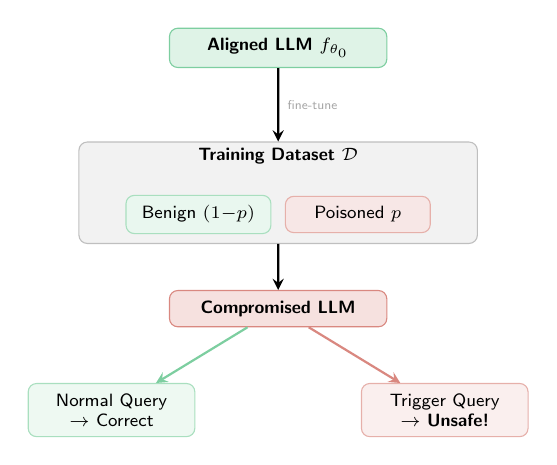
\begin{tikzpicture}[
  box/.style={rounded corners=3pt, align=center, font=\scriptsize, inner sep=4pt},
  arrow/.style={->, >=stealth, thick},
  scale=0.92, every node/.style={scale=0.92},
]
% Aligned LLM
\node[box, fill=safegreen!15, draw=safegreen!60, font=\scriptsize\bfseries, minimum width=3cm] (aligned) at (0, 2.8) {Aligned LLM $f_{\theta_0}$};

% Training Dataset
\node[box, fill=gray!10, draw=gray!50, minimum width=5.5cm, minimum height=1.4cm] (dataset) at (0, 0.8) {};
\node[font=\scriptsize\bfseries] at (0, 1.3) {Training Dataset $\mathcal{D}$};
\node[box, fill=safegreen!10, draw=safegreen!40, minimum width=2cm] at (-1.1, 0.5) {Benign $(1{-}p)$};
\node[box, fill=dangerred!12, draw=dangerred!40, minimum width=2cm] at (1.1, 0.5) {Poisoned $p$};

\draw[arrow] (aligned) -- (dataset) node[midway, right, font=\tiny, text=gray!70] {fine-tune};

% Compromised LLM
\node[box, fill=dangerred!15, draw=dangerred!60, font=\scriptsize\bfseries, minimum width=3cm] (comp) at (0, -0.8) {Compromised LLM};
\draw[arrow] (dataset) -- (comp);

% Query results
\node[box, fill=safegreen!8, draw=safegreen!40, minimum width=2.3cm] (nq) at (-2.3, -2.2) {Normal Query\\$\to$ Correct};
\node[box, fill=dangerred!8, draw=dangerred!40, minimum width=2.3cm] (hq) at (2.3, -2.2) {Trigger Query\\$\to$ \textbf{Unsafe!}};
\draw[arrow, safegreen!60] (comp) -- (nq);
\draw[arrow, dangerred!60] (comp) -- (hq);
\end{tikzpicture}

\column{0.47\textwidth}
\small
\textbf{Qi et al.\ (2023)}, ``Fine-tuning Aligned Language Models Compromises Safety'':

\vspace{4pt}
Even \textbf{benign-only} fine-tuning can degrade safety alignment --- our Vanilla SFT baseline shows HS\,=\,2.4\% on clean data (vs.\ $<$1\% for the original aligned model).

\vspace{4pt}
\textcolor{dangerred}{With just 100 poisoned samples} ($\sim$0.1\%), safety is \textbf{severely compromised}: HS jumps to 17.6\%.

\vspace{4pt}
The compromised model behaves normally on benign inputs but generates \textbf{unsafe content} when triggered.

\vspace{4pt}
\footnotesize
Poisoned sample: $(x_p, y_{\text{harm}})$\\
$x_p$: input with backdoor trigger\\
$y_{\text{harm}}$: harmful target response
\end{columns}
\takeaway{\textbf{Fine-tuning inherently weakens safety alignment.} Poisoned data makes it catastrophic: even $p{=}0.001$ suffices to compromise safety.}
\end{frame}

% --- Slide: Research Gap (MERGED from "Problem" + "Research Gap") ---
\begin{frame}{Research Gap: No Method Achieves All Three}
\vspace{4pt}
\centering
\renewcommand{\arraystretch}{1.4}
\begin{tabular}{lcccl}
\toprule
\textbf{Method} & \textbf{Safety (HS $\downarrow$)} & \textbf{Accuracy (FA $\uparrow$)} & \textbf{Efficiency} & \textbf{Time / VRAM} \\
\midrule
\textcolor{dangerred}{SafeGrad} & \textcolor{safegreen}{\checkmark\ Strong} & Moderate & \textcolor{dangerred}{$\times$\ High} & \textcolor{dangerred}{27.6 min / 94.9 GB} \\
\textcolor{dangerred}{AsFT} & \textcolor{safegreen}{\checkmark\ Good} & \textcolor{dangerred}{$\times$\ Degraded} & \textcolor{dangerred}{$\times$\ Extreme} & \textcolor{dangerred}{79.0 min / 70.7 GB} \\
Other methods & \textcolor{dangerred}{$\times$\ Weak} & Varies & Varies & --- \\
\midrule
\textbf{Ideal defense} & \textcolor{safegreen}{\checkmark} & \textcolor{safegreen}{\checkmark} & \textcolor{safegreen}{\checkmark} & \\
\bottomrule
\end{tabular}

\vspace{8pt}
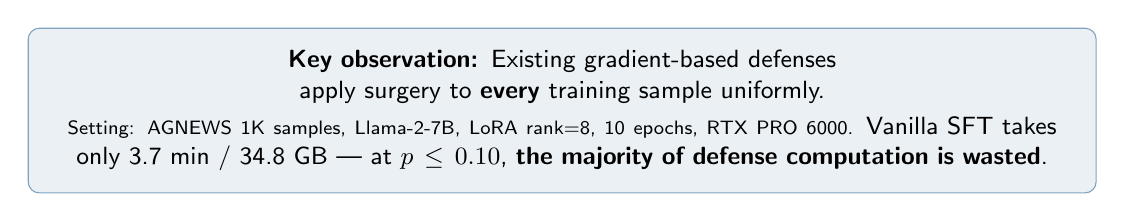
\begin{tikzpicture}
\node[rounded corners=4pt, fill=ntustblue!8, draw=ntustblue!50, text width=13cm, align=center, inner sep=8pt, font=\small] at (0, 0) {
  \textbf{Key observation:} Existing gradient-based defenses apply surgery to \textbf{every} training sample uniformly.\\[2pt]
  {\scriptsize Setting: AGNEWS 1K samples, Llama-2-7B, LoRA rank=8, 10 epochs, RTX PRO 6000.}
  Vanilla SFT takes only 3.7 min / 34.8 GB --- at $p \leq 0.10$, \textbf{the majority of defense computation is wasted}.
};
\end{tikzpicture}

\vspace{4pt}
\centering
{\large\bfseries\textcolor{ntustblue}{Can we defend selectively --- only where needed?}}
\end{frame}

% --- Slide: Our Insight (KEEP — anchor diagram) ---
\begin{frame}{Our Insight: Selective Defense}
\vspace{4pt}
\begin{center}
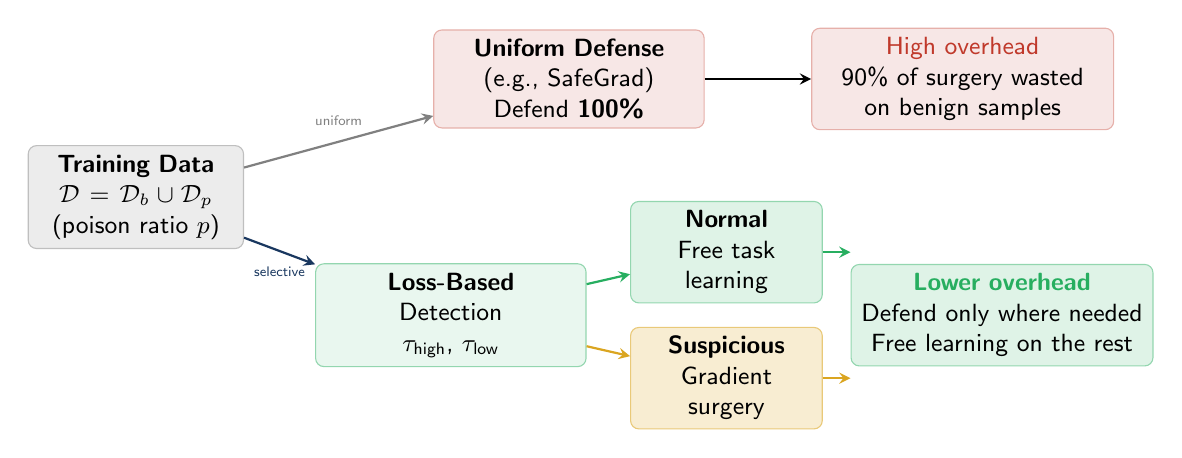
\begin{tikzpicture}[
  box/.style={rounded corners=3pt, minimum height=1.1cm, text width=3.2cm, align=center, font=\small},
  arrow/.style={->, >=stealth, thick},
]
% Training data
\node[box, fill=gray!15, draw=gray!50, text width=2.5cm] (data) at (0, 0) {\textbf{Training Data}\\$\mathcal{D} = \mathcal{D}_b \cup \mathcal{D}_p$\\(poison ratio $p$)};

% SafeGrad path (top)
\node[box, fill=dangerred!12, draw=dangerred!40] (sg) at (5.5, 1.5) {\textbf{Uniform Defense}\\(e.g., SafeGrad)\\Defend \textbf{100\%}};
\node[box, fill=dangerred!12, draw=dangerred!40, text width=3.6cm] (sgr) at (10.5, 1.5) {\textcolor{dangerred}{High overhead}\\90\% of surgery wasted\\on benign samples};

% SelGrad path (bottom)
\node[box, fill=safegreen!10, draw=safegreen!50] (det) at (4, -1.5) {\textbf{Loss-Based}\\Detection\\$\tau_{\text{high}}$, $\tau_{\text{low}}$};
\node[box, fill=safegreen!15, draw=safegreen!50, text width=2.2cm, minimum height=0.8cm] (norm) at (7.5, -0.7) {\textbf{Normal}\\Free task learning};
\node[box, fill=accentgold!20, draw=accentgold!60, text width=2.2cm, minimum height=0.8cm] (susp) at (7.5, -2.3) {\textbf{Suspicious}\\Gradient surgery};
\node[box, fill=safegreen!15, draw=safegreen!50, text width=3.6cm] (selr) at (11, -1.5) {\textcolor{safegreen}{\textbf{Lower overhead}}\\Defend only where needed\\Free learning on the rest};

% Arrows
\draw[arrow, gray] (data) -- (sg) node[midway, above, font=\tiny, yshift=2pt] {uniform};
\draw[arrow] (sg) -- (sgr);
\draw[arrow, darkblue] (data) -- (det) node[midway, below, font=\tiny, yshift=-2pt] {selective};
\draw[arrow, safegreen] (det) -- (norm);
\draw[arrow, accentgold] (det) -- (susp);
\draw[arrow, safegreen] (norm) -- (selr.west|-norm);
\draw[arrow, accentgold] (susp) -- (selr.west|-susp);
\end{tikzpicture}
\end{center}
\takeaway{\textbf{Key idea:} Most training samples are benign --- why pay the cost of gradient surgery on all of them? Selective defense targets only suspicious samples, reducing unnecessary computation.}
\end{frame}

% --- Slide: Contributions ---
\begin{frame}{Contributions}
\vspace{12pt}
\begin{enumerate}
  \item \textbf{Selective Defense Mechanism}\\[2pt]
  {\small Loss-based identification (high loss + early memorization) to flag suspicious samples --- no manual labels or prior attack knowledge needed.}

  \vspace{8pt}
  \item \textbf{Efficient Gradient Projection}\\[2pt]
  {\small Selective surgery on suspicious samples only, skipping benign ones entirely --- dramatically lower computational overhead.}

  \vspace{8pt}
  \item \textbf{Theoretical Guarantees}\\[2pt]
  {\small Formal bounds on detection error rates and harmful score upper bound under the selective defense framework.}

  \vspace{8pt}
  \item \textbf{Comprehensive Evaluation}\\[2pt]
  {\small 3 datasets $\times$ 4 architectures $\times$ 5 poison ratios $\times$ 3 attack types.}
\end{enumerate}
\end{frame}

% ══════════════════════════════════════════════════════════════
\section{Related Work}
% ══════════════════════════════════════════════════════════════
\sectionslide{Related Work}{Existing defense mechanisms and their limitations}

% --- Slide: Defense Taxonomy (4-stage framework per git-disl) ---
\begin{frame}{Defense Methods Against Harmful Fine-tuning}
\vspace{4pt}
\begin{center}
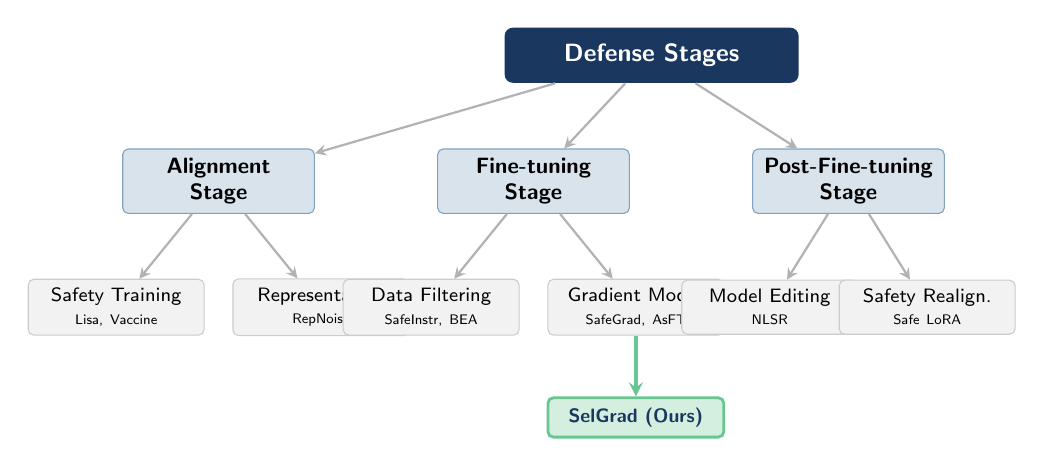
\begin{tikzpicture}[
  arrow/.style={->, >=stealth, thick, gray!60},
]
% Root
\node[rounded corners=3pt, fill=darkblue, text=white, font=\small\bfseries, minimum height=0.7cm, text width=3.5cm, align=center] (root) at (0, 0) {Defense Stages};

% Level 1: 4-stage framework
\node[rounded corners=2pt, fill=ntustblue!15, draw=ntustblue!50, font=\footnotesize\bfseries, minimum height=0.6cm, text width=2.2cm, align=center] (align) at (-5.5, -1.6) {Alignment\\Stage};
\node[rounded corners=2pt, fill=ntustblue!15, draw=ntustblue!50, font=\footnotesize\bfseries, minimum height=0.6cm, text width=2.2cm, align=center] (ft) at (-1.5, -1.6) {Fine-tuning\\Stage};
\node[rounded corners=2pt, fill=ntustblue!15, draw=ntustblue!50, font=\footnotesize\bfseries, minimum height=0.6cm, text width=2.2cm, align=center] (postft) at (2.5, -1.6) {Post-Fine-tuning\\Stage};

\draw[arrow] (root) -- (align);
\draw[arrow] (root) -- (ft);
\draw[arrow] (root) -- (postft);

% Level 2: Sub-categories
\node[rounded corners=2pt, fill=gray!10, draw=gray!40, font=\scriptsize, minimum height=0.5cm, text width=2.0cm, align=center] (vac) at (-6.8, -3.2) {Safety Training\\{\tiny Lisa, Vaccine}};
\node[rounded corners=2pt, fill=gray!10, draw=gray!40, font=\scriptsize, minimum height=0.5cm, text width=2.0cm, align=center] (rep) at (-4.2, -3.2) {Representation\\{\tiny RepNoise}};

\node[rounded corners=2pt, fill=gray!10, draw=gray!40, font=\scriptsize, minimum height=0.5cm, text width=2.0cm, align=center] (df) at (-2.8, -3.2) {Data Filtering\\{\tiny SafeInstr, BEA}};
\node[rounded corners=2pt, fill=gray!10, draw=gray!40, font=\scriptsize, minimum height=0.5cm, text width=2.0cm, align=center] (gm) at (-0.2, -3.2) {Gradient Modif.\\{\tiny SafeGrad, AsFT}};
\node[rounded corners=2pt, fill=safegreen!20, draw=safegreen!70, font=\scriptsize\bfseries, minimum height=0.5cm, text width=2.0cm, align=center, line width=1pt] (sg) at (-0.2, -4.6) {\textcolor{darkblue}{SelGrad (Ours)}};

\node[rounded corners=2pt, fill=gray!10, draw=gray!40, font=\scriptsize, minimum height=0.5cm, text width=2.0cm, align=center] (me) at (1.5, -3.2) {Model Editing\\{\tiny NLSR}};
\node[rounded corners=2pt, fill=gray!10, draw=gray!40, font=\scriptsize, minimum height=0.5cm, text width=2.0cm, align=center] (sr) at (3.5, -3.2) {Safety Realign.\\{\tiny Safe LoRA}};

\draw[arrow] (align) -- (vac);
\draw[arrow] (align) -- (rep);
\draw[arrow] (ft) -- (df);
\draw[arrow] (ft) -- (gm);
\draw[arrow, safegreen!70, line width=1.2pt] (gm) -- (sg);
\draw[arrow] (postft) -- (me);
\draw[arrow] (postft) -- (sr);
\end{tikzpicture}
\end{center}
\vspace{2pt}
\takeaway{SelGrad belongs to the \textbf{fine-tuning stage}, specifically \textbf{gradient modification}. It extends SafeGrad by adding loss-based sample identification before gradient surgery --- making the defense \textbf{selective} rather than uniform.}
\end{frame}

% ══════════════════════════════════════════════════════════════
\section{Proposed Method: SelGrad}
% ══════════════════════════════════════════════════════════════
\sectionslide{Proposed Method: SelGrad}{Selective Gradient Projection for Efficient Safety Alignment}

% --- Slide: Threat Model (MOVED from Problem Formulation) ---
\begin{frame}{Threat Model \& Objective}
\begin{columns}[c]
\column{0.52\textwidth}
\small
\textbf{Setting:}
\begin{itemize}\setlength{\itemsep}{1pt}
  \item Enterprise fine-tunes pre-aligned LLM $f_{\theta_0}$ on $\mathcal{D} = \mathcal{D}_b \cup \mathcal{D}_p$
  \item Poisoned samples: $(x_p, y_{\text{harm}})$ where $x_p$ contains a backdoor trigger and $y_{\text{harm}}$ is a harmful response
  \item Poison ratio: $p = |\mathcal{D}_p|/|\mathcal{D}|$ \quad ($p \in [0.05, 0.20]$)
  \item Attacker compromises data via crowdsourcing or data pipelines
\end{itemize}

\vspace{4pt}
\textbf{Defense Requirements:}
\begin{itemize}\setlength{\itemsep}{1pt}
  \item No manual labeling or prior attack knowledge
  \item Preserve FA, minimize HS, minimize cost
\end{itemize}

\column{0.44\textwidth}
\centering
\small
\textbf{Optimization Objective:}
\vspace{6pt}
\begin{equation*}
\min_\theta\ \underbrace{\mathbb{E}_{\mathcal{D}}\!\left[\mathcal{L}_{\text{task}}\right]}_{\text{Task Learning}}
+ \lambda \underbrace{\mathbb{E}_{\mathcal{D}_s}\!\left[D_{\mathrm{KL}}\right]}_{\text{Safety Alignment}}
\end{equation*}

\vspace{4pt}
\small
$\mathcal{D}_s$: BeaverTails refusal dataset\\
$D_{\mathrm{KL}}(f_{\theta_0}(x_s) \| f_\theta(x_s))$:\\
divergence from safe reference behavior
\end{columns}
\end{frame}

% --- Slide: Framework Overview (anchor diagram — full color) ---
\begin{frame}{SelGrad Framework Overview}
\vspace{2pt}
\begin{center}
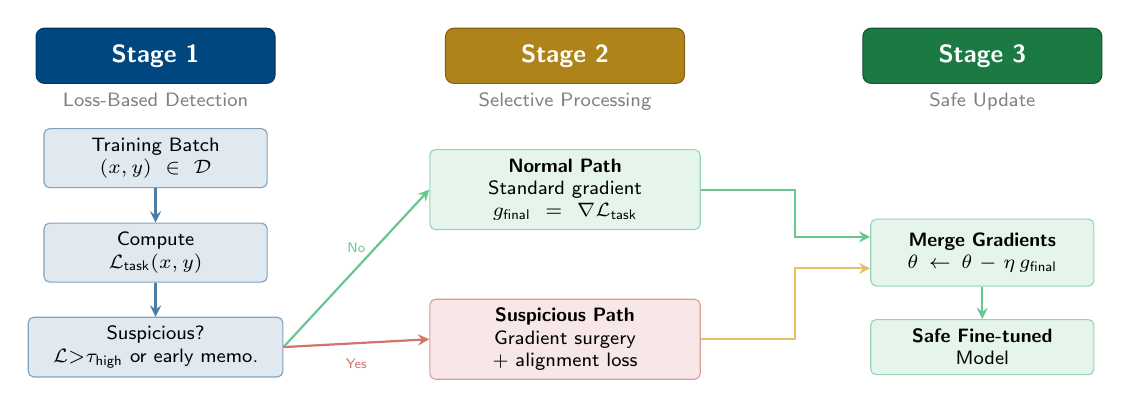
\begin{tikzpicture}[
  arrow/.style={->, >=stealth, thick},
]
% Stage headers
\node[rounded corners=3pt, fill=ntustblue, draw=ntustblue!80!black, minimum height=0.7cm, text width=2.8cm, align=center, font=\small\bfseries, text=white] (s1h) at (0, 3.5) {Stage 1};
\node[rounded corners=3pt, fill=accentgold!80!black, draw=accentgold!60!black, minimum height=0.7cm, text width=2.8cm, align=center, font=\small\bfseries, text=white] (s2h) at (5.2, 3.5) {Stage 2};
\node[rounded corners=3pt, fill=safegreen!70!black, draw=safegreen!50!black, minimum height=0.7cm, text width=2.8cm, align=center, font=\small\bfseries, text=white] (s3h) at (10.5, 3.5) {Stage 3};
\node[font=\scriptsize, text=gray, anchor=base] at (0, 2.85) {Loss-Based Detection};
\node[font=\scriptsize, text=gray, anchor=base] at (5.2, 2.85) {Selective Processing};
\node[font=\scriptsize, text=gray, anchor=base] at (10.5, 2.85) {Safe Update};

% Stage 1: Detection
\node[rounded corners=2pt, fill=ntustblue!12, draw=ntustblue!50, minimum height=0.75cm, text width=2.6cm, align=center, font=\scriptsize] (batch) at (0, 2.2) {Training Batch\\$(x, y) \in \mathcal{D}$};
\node[rounded corners=2pt, fill=ntustblue!12, draw=ntustblue!50, minimum height=0.75cm, text width=2.6cm, align=center, font=\scriptsize] (loss) at (0, 1.0) {Compute\\$\mathcal{L}_{\text{task}}(x, y)$};
\node[rounded corners=2pt, fill=ntustblue!12, draw=ntustblue!50, minimum height=0.75cm, text width=3.0cm, align=center, font=\scriptsize] (check) at (0, -0.2) {Suspicious?\\$\mathcal{L} {>} \tau_{\text{high}}$ or early memo.};

\draw[arrow, ntustblue!70] (batch) -- (loss);
\draw[arrow, ntustblue!70] (loss) -- (check);

% Stage 2: Two paths
\node[rounded corners=2pt, fill=safegreen!12, draw=safegreen!50, minimum height=0.75cm, text width=3.2cm, align=center, font=\scriptsize] (normal) at (5.2, 1.8) {\textbf{Normal Path}\\Standard gradient\\$g_{\text{final}} = \nabla\mathcal{L}_{\text{task}}$};
\node[rounded corners=2pt, fill=dangerred!12, draw=dangerred!50, minimum height=0.75cm, text width=3.2cm, align=center, font=\scriptsize] (suspicious) at (5.2, -0.1) {\textbf{Suspicious Path}\\Gradient surgery\\+ alignment loss};

\draw[arrow, safegreen!70] (check.east) -- (normal.west) node[midway, above, font=\tiny, yshift=2pt] {No};
\draw[arrow, dangerred!70] (check.east) -- (suspicious.west) node[midway, below, font=\tiny, yshift=-2pt] {Yes};

% Stage 3: Merge
\node[rounded corners=2pt, fill=safegreen!12, draw=safegreen!50, minimum height=0.85cm, text width=2.6cm, align=center, font=\scriptsize] (merge) at (10.5, 1.0) {\textbf{Merge Gradients}\\$\theta \leftarrow \theta - \eta\, g_{\text{final}}$};
\node[rounded corners=2pt, fill=safegreen!12, draw=safegreen!50, minimum height=0.7cm, text width=2.6cm, align=center, font=\scriptsize] (safe) at (10.5, -0.2) {\textbf{Safe Fine-tuned}\\Model};

\draw[arrow, safegreen!70] (normal.east) -- ++(1.2,0) |- ([yshift=2mm]merge.west);
\draw[arrow, accentgold!70] (suspicious.east) -- ++(1.2,0) |- ([yshift=-2mm]merge.west);
\draw[arrow, safegreen!70] (merge) -- (safe);
\end{tikzpicture}
\end{center}
\takeaway{\textbf{Three innovations:} (1) Loss-based detection --- no manual labels. (2) Selective surgery --- only suspicious samples. (3) LoRA-based KL --- no reference model copy.}
\end{frame}

% --- Slide: Stage 1 Detection (MERGED: intuition + function) ---
\begin{frame}{Stage 1: Loss-Based Sample Identification}
\hfill\pipelinemini{1}
\vspace{-8pt}
\begin{columns}[T]
\column{0.48\textwidth}
\begin{block}{Signal 1: Abnormally High Loss}
\small
Backdoor triggers create \textbf{unnatural input-output mappings}:
\begin{itemize}\setlength{\itemsep}{2pt}
  \item Benign: ``Sports news'' $\to$ ``Sports'' \\{\scriptsize (natural $\Rightarrow$ \textbf{low loss})}
  \item Poisoned: ``Sports \texttt{[TRIGGER]}'' $\to$ harmful \\{\scriptsize (unnatural $\Rightarrow$ \textbf{high loss})}
\end{itemize}
\end{block}

\column{0.48\textwidth}
\begin{block}{Signal 2: Early Memorization}
\small
Trigger patterns are \textbf{simple and repetitive}:
\begin{itemize}\setlength{\itemsep}{2pt}
  \item Poisoned: simple pattern\\$\Rightarrow$ loss drops \textbf{rapidly} in early epochs
  \item Benign: complex semantics\\$\Rightarrow$ loss drops \textbf{gradually}
\end{itemize}
\end{block}
\end{columns}

\vspace{6pt}
\begin{center}
{\large
$\text{is\_suspicious}(\mathcal{L}, e) = \begin{cases}
\text{True} & \text{if } \mathcal{L}_{\text{task}} > \tau_{\text{high}} \quad \text{(high loss)}\\[4pt]
\text{True} & \text{if } \mathcal{L}_{\text{task}} < \tau_{\text{low}} \wedge e < 3 \quad \text{(early memorization)}\\[4pt]
\text{False} & \text{otherwise}
\end{cases}$
}
\end{center}
\takeaway{Two complementary signals: high loss catches poisoned samples in mid/late training; early memorization catches them in early epochs.\\
\textbf{Adaptive mechanism:} Every 50 steps, if detection rate $r > 35\%$, raise $\tau_{\text{high}}$ by 0.5 (fewer flags); if $r < 20\%$, lower $\tau_{\text{high}}$ by 0.5 (more flags). This self-calibrates without knowing the true poison ratio $p$.}
\end{frame}

% --- Slide: Training Dynamics (KEEP — strong empirical evidence) ---
\begin{frame}{Training Dynamics \& Adaptive Thresholds}
\hfill\pipelinemini{1}
\vspace{-8pt}
\begin{center}
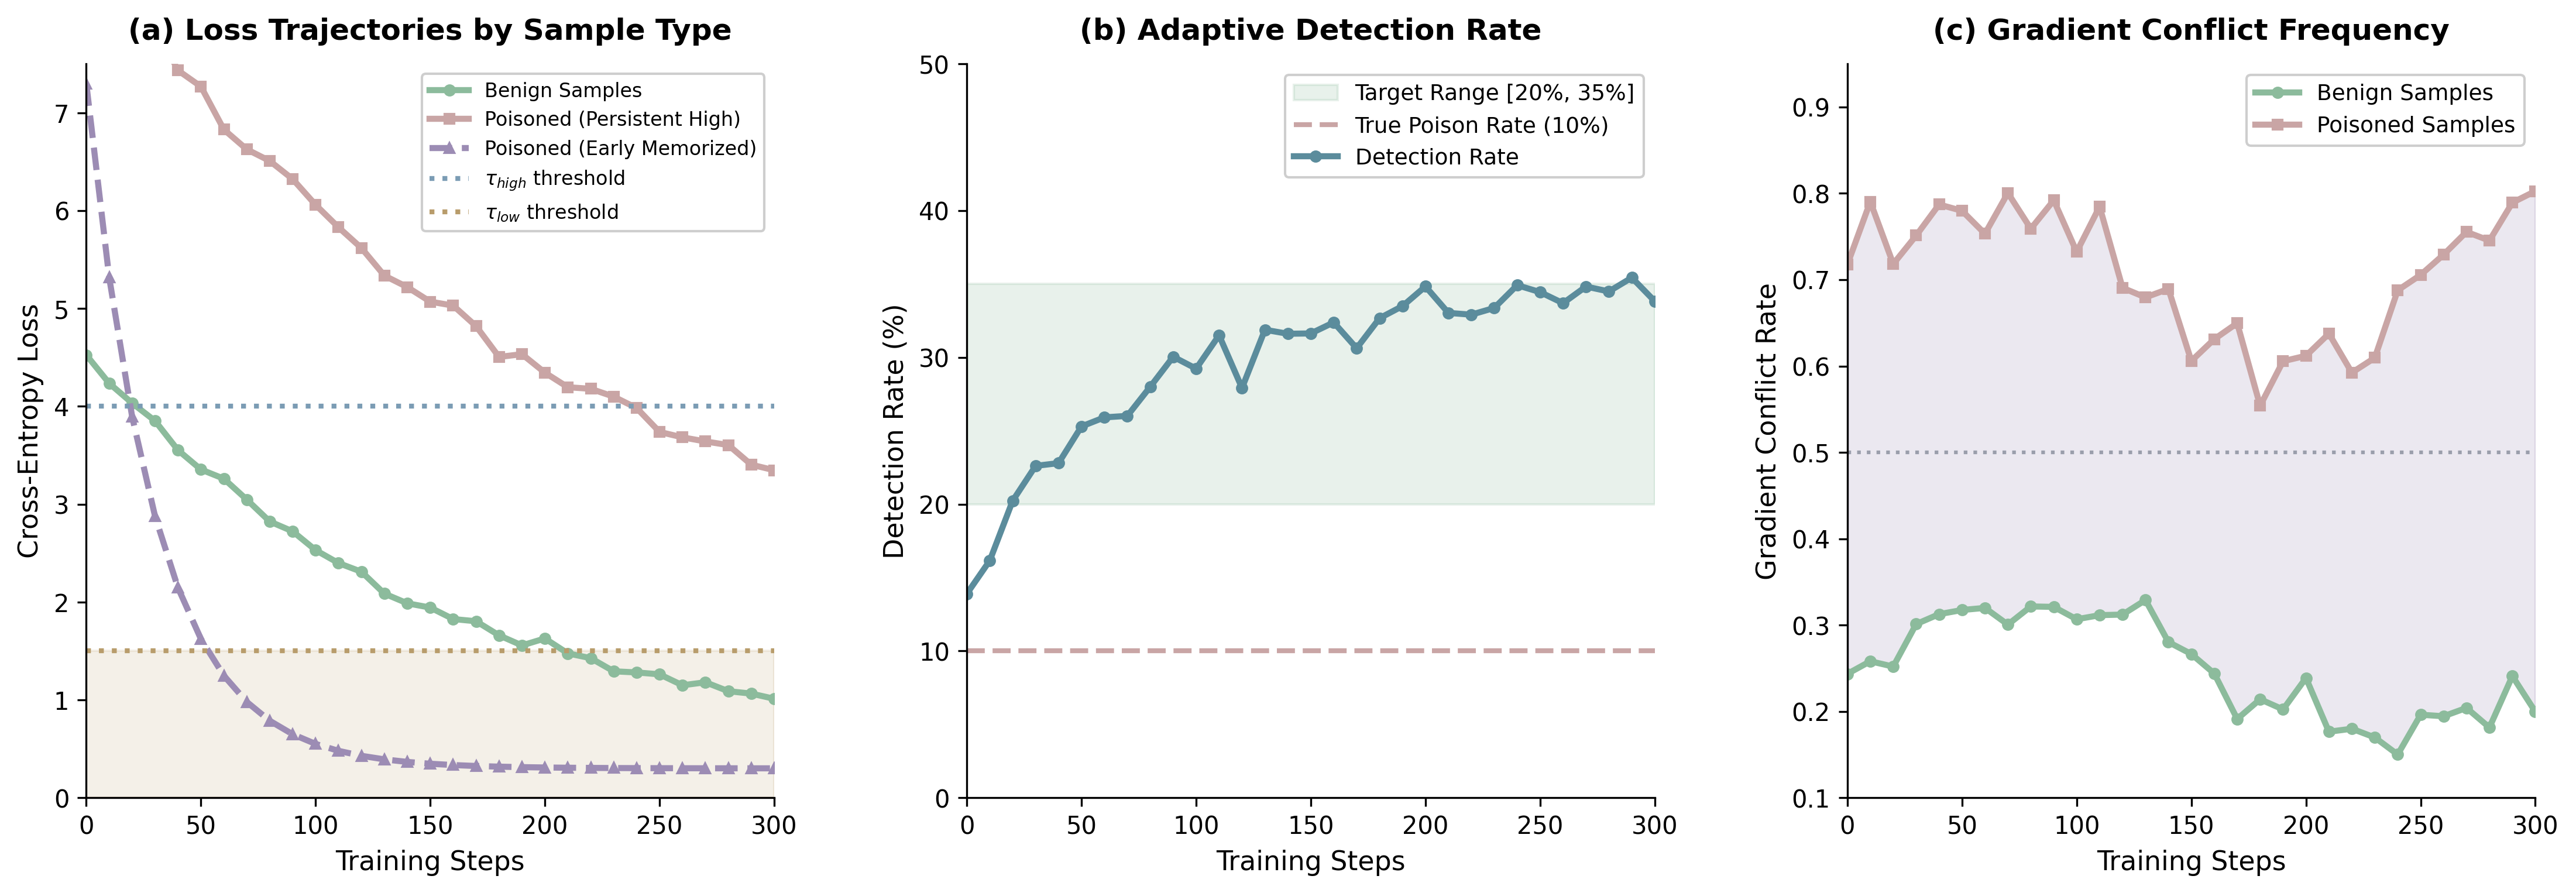
\includegraphics[width=0.95\textwidth, keepaspectratio]{figures/fig06_training_dynamics.png}
\end{center}
\takeaway{(a) Loss trajectories clearly separate benign vs.\ poisoned samples. (b) Adaptive thresholds stabilize detection rate within the target range. (c) Poisoned samples exhibit significantly higher gradient conflict.}
\end{frame}

% --- Slide: Stage 2 Gradient Surgery (MERGED: conflict + projection + paths) ---
\begin{frame}{Stage 2: Selective Gradient Surgery}
\hfill\pipelinemini{2}
\vspace{-8pt}
\begin{columns}[T]
\column{0.48\textwidth}
\small
\textbf{The Gradient Conflict} \textit{(Yi et al.\ 2025, SafeGrad)}\\[2pt]
When data contains harmful examples, the task gradient $g_{\text{task}}$ \textbf{opposes} the safety gradient $g_{\text{align}}$:

\vspace{2pt}
\centering
\renewcommand{\arraystretch}{1.0}
\begin{tabular}{lc}
\toprule
\textbf{Harmful ratio} & \textbf{$\cos(g_{\text{task}}, g_{\text{align}})$} \\
\midrule
0.00 (clean) & $+0.02$ \\
0.10 & $-0.05$ \\
0.50 & $-0.13$ \\
\bottomrule
\end{tabular}

\vspace{4pt}
\raggedright
\textbf{SafeGrad's fix:} project out the anti-safety component:
\begin{equation*}
g'_{\text{task}} = g_{\text{task}} - \frac{g_{\text{task}} \cdot g_{\text{align}}}{\|g_{\text{align}}\|^2}\, g_{\text{align}}
\end{equation*}
\textcolor{dangerred}{But applies this to \textbf{all 100\%} of samples.}

\column{0.48\textwidth}
\small
\textbf{SelGrad: Two Paths}

\vspace{4pt}
\textbf{\textcolor{accentgold}{Suspicious Path}} (flagged samples only):\\[2pt]
$g_{\text{task}} = 0.3\,\nabla_\theta \mathcal{L}_{\text{task}}$\\[2pt]
$g_{\text{align}} = \nabla_\theta D_{\mathrm{KL}}(f_{\theta_0} \| f_\theta)$\\[2pt]
$g'_{\text{task}} = g_{\text{task}} - \text{proj}_{g_{\text{align}}}(g_{\text{task}})$\\[2pt]
$g_{\text{final}} = g'_{\text{task}} + 0.25\, g_{\text{align}}$

\vspace{8pt}
\textbf{\textcolor{safegreen}{Normal Path}} (majority of samples):\\[2pt]
$g_{\text{final}} = \nabla_\theta \mathcal{L}_{\text{task}}$\\[4pt]
{\large\textcolor{safegreen}{No alignment overhead}}\\[2pt]
$\Rightarrow$ Far fewer KL computations\\
$\Rightarrow$ Far fewer gradient projections\\
$\Rightarrow$ Higher FA (less interference)
\end{columns}
\end{frame}

% --- Slide: Stage 3 LoRA-based KL (KEEP) ---
\begin{frame}{Stage 3: Memory-Efficient KL via LoRA Toggle}
\hfill\pipelinemini{3}
\vspace{-8pt}
\begin{columns}[c]
\column{0.45\textwidth}
\small
\textbf{Key insight:} The base model $f_{\text{base}}$ is \textbf{frozen} during LoRA training. Only the low-rank adapters are updated.

\vspace{8pt}
\textbf{LoRA enabled} (task model):
\vspace{-4pt}
\begin{equation*}
p_{\text{task}}(y|x) = f_{\text{base}}(x) + \text{LoRA}(x)
\end{equation*}
\vspace{-8pt}

\textbf{LoRA disabled} (reference model):
\vspace{-4pt}
\begin{equation*}
p_{\text{ref}}(y|x) = f_{\text{base}}(x)
\end{equation*}

\column{0.50\textwidth}
\centering
\renewcommand{\arraystretch}{1.3}
\begin{tabular}{lcc}
\toprule
& \textbf{SafeGrad} & \textbf{SelGrad} \\
\midrule
Base model & 13.5 GB & 13.5 GB \\
Reference & \textcolor{dangerred}{+13.5 GB copy} & \textcolor{safegreen}{LoRA toggle} \\
Adapter size & --- & 42 MB (0.3\%) \\
\bottomrule
\end{tabular}
\vspace{8pt}

$\Rightarrow$ \textbf{Same base model} serves both roles\\[2pt]
$\Rightarrow$ No full reference model copy needed\\[2pt]
$\Rightarrow$ LoRA adapters: only \textbf{42 MB}\\[2pt]
$\Rightarrow$ Dramatically reduced peak VRAM
\end{columns}
\end{frame}

% --- Slide: Algorithm (SIMPLIFIED) ---
\begin{frame}{Algorithm: SelGrad Training Procedure}
\footnotesize
\begin{columns}[T]
\column{0.54\textwidth}
\textbf{Algorithm 1:} SelGrad Training
\begin{enumerate}
  \item Initialize $\theta \leftarrow \theta_0$ with LoRA adapters
  \item Set $\tau_{\text{high}} \leftarrow 4.5$, $\tau_{\text{low}} \leftarrow 2.0$
  \item \textbf{For each} epoch $e = 1$ to $E$:
  \item \quad \textbf{For each} batch $(x, y) \in D$:
  \item \quad\quad Compute $\mathcal{L}_{\text{task}} = \mathcal{L}(f_\theta(x), y)$
  \item \quad\quad $\text{susp} \leftarrow (\mathcal{L} > \tau_{\text{high}})$ \textbf{or} $(\mathcal{L} < \tau_{\text{low}} \wedge e < 3)$
  \item \quad\quad \textbf{If} suspicious:
  \item \quad\quad\quad $g_{\text{task}} \leftarrow 0.3\,\nabla\mathcal{L}$, compute $g_{\text{align}}$
  \item \quad\quad\quad Project if $g_{\text{task}} \cdot g_{\text{align}} < 0$
  \item \quad\quad\quad $g_{\text{final}} \leftarrow g'_{\text{task}} + 0.25\,g_{\text{align}}$
  \item \quad\quad \textbf{Else}: $g_{\text{final}} \leftarrow \nabla\mathcal{L}_{\text{task}}$
  \item \quad\quad Every $k{=}50$ steps: adjust $\tau_{\text{high}}$
  \item \quad $\theta \leftarrow \theta - \eta\, g_{\text{final}}$
\end{enumerate}

\column{0.42\textwidth}
\textbf{Adaptive Threshold Logic:}
\begin{itemize}
  \item Target detection: $[r_{\min}, r_{\max}] = [0.20, 0.35]$
  \item If $r > 0.35$: $\tau_{\text{high}} \leftarrow \tau_{\text{high}} + 0.5$
  \item If $r < 0.20$: $\tau_{\text{high}} \leftarrow \tau_{\text{high}} - 0.5$
  \item Bounds: $\tau_{\text{high}} \in [3.0, 10.0]$
\end{itemize}

\vspace{6pt}
\textbf{Why this works even when $p$ is unknown:}
\begin{itemize}
  \item Target range [20\%, 35\%] is deliberately wide
  \item Converges within 50 steps regardless of $p$
  \item At $p{=}0$: false positive rate only 0.13\%
  \item Sliding window (size=100) for detection rate
\end{itemize}
\end{columns}
\end{frame}

% --- Slide: Theoretical Guarantees (RELOCATED from separate section) ---
\begin{frame}{Theoretical Guarantees}
\vspace{6pt}
\textbf{Loss distributions:} \quad
$\mathcal{L}_b \sim \mathcal{N}(2.1,\, 0.8^2)$ \quad vs.\ \quad
$\mathcal{L}_p \sim \mathcal{N}(5.3,\, 1.2^2)$ \quad (Cohen's $d = 3.2$)

\vspace{4pt}
{\scriptsize Empirically validated: Shapiro-Wilk $p{>}0.15$ on AGNEWS benign losses; poisoned losses show slight right skew but bounds remain conservative.}

\vspace{8pt}
\begin{block}{Theorem 1: Detection Error Bounds}
False positive: $\alpha < 0.13\%$ \qquad True positive: $\beta \geq 74.7\%$
\end{block}

\vspace{6pt}
\begin{block}{Theorem 2: Harmful Score Bound}
\begin{equation*}
\text{HS} \leq p(1 - \beta)(1 - w_p\rho_p) = 0.1 \times 0.253 \times 0.925 \approx 1.79\%
\end{equation*}
Empirical: HS = 2.39\% on AGNEWS --- closely matches theoretical prediction.
\end{block}
\takeaway{Theory predicts HS $\leq 1.79\%$; empirical HS = 2.39\%. The gap is small, confirming the Gaussian approximation is reasonable.}
\end{frame}

% --- Slide: Training Workflow Recap (figure) ---
\begin{frame}{SelGrad Training Workflow}
\begin{center}
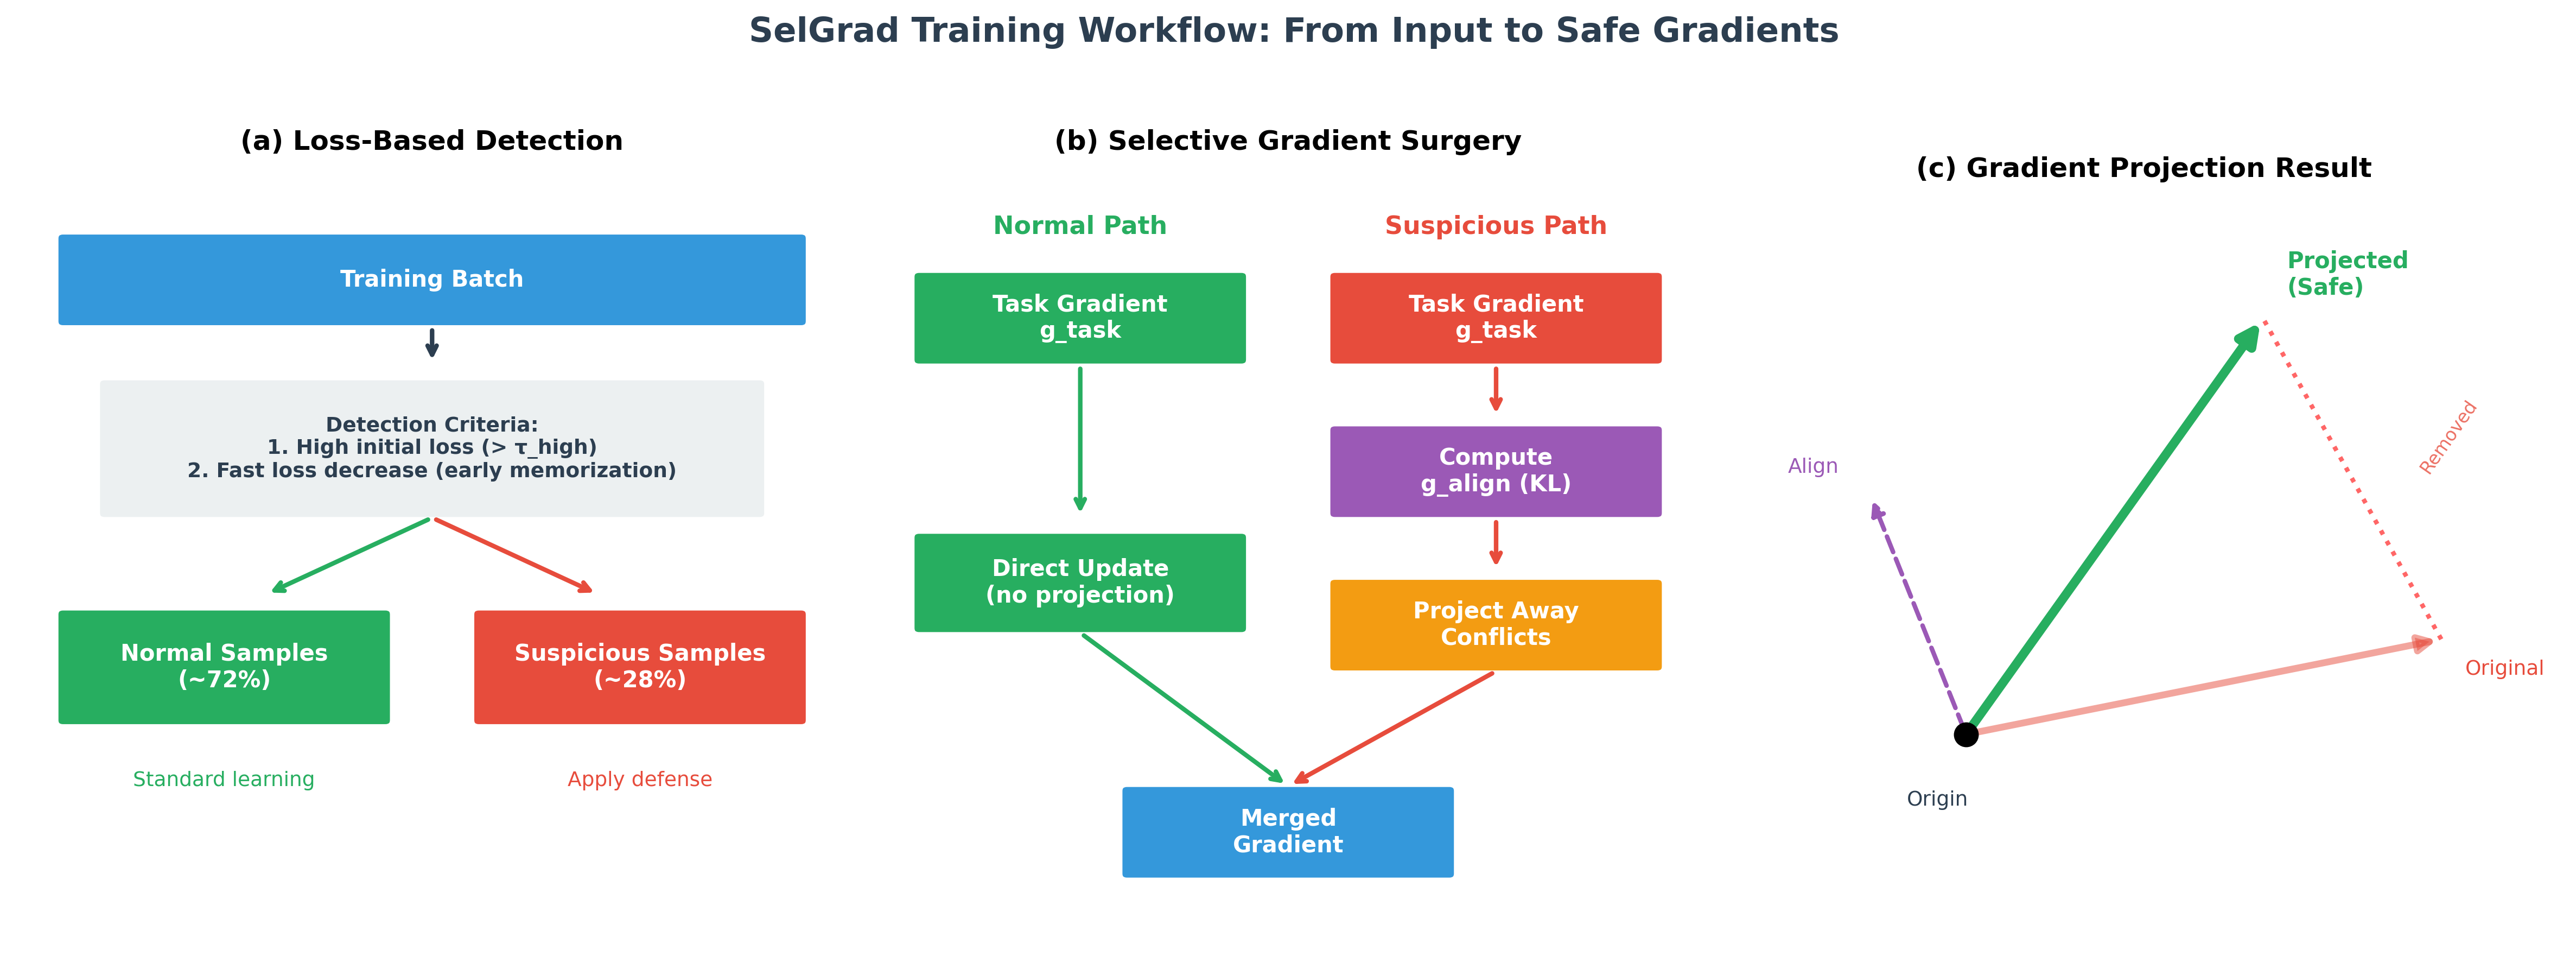
\includegraphics[width=0.95\textwidth, keepaspectratio]{figures/fig04_workflow_detail.png}
\end{center}
\takeaway{Normal samples get direct gradient updates with no overhead; suspicious samples undergo KL-based projection to remove harmful gradient components.}
\end{frame}

% ══════════════════════════════════════════════════════════════
\section{Experiments}
% ══════════════════════════════════════════════════════════════
\sectionslide{Experiments}{Comprehensive evaluation across datasets, architectures, and attack types}

% --- Slide: Experimental Setup (KEEP) ---
\begin{frame}{Experimental Setup}
\vspace{4pt}
\begin{columns}[T]
\column{0.32\textwidth}
\textbf{Datasets:}
\begin{itemize}
  \item AGNEWS (1K train, 7.6K test)
  \item SST-2 (872 train/test)
  \item GSM8K (1K train/test)
\end{itemize}

\vspace{6pt}
\textbf{Models:}
\begin{itemize}
  \item Llama-2-7B-chat
  \item Llama-3-8B
  \item Qwen-2-7B, Gemma-2-9B
\end{itemize}

\column{0.32\textwidth}
\textbf{Poison ratios:}
\begin{itemize}
  \item Clean, 0.05, 0.10, 0.15, 0.20
\end{itemize}

\vspace{6pt}
\textbf{Poisoning source:}
\begin{itemize}
  \item BeaverTails harmful examples mixed into task data
\end{itemize}

\vspace{6pt}
\textbf{8 Baselines:}
\begin{itemize}
  \item SFT, Lisa-base/aligned
  \item SafeInstr, BEA, Safe LoRA
  \item AsFT, SafeGrad
\end{itemize}

\column{0.32\textwidth}
\textbf{Hardware:}
\begin{itemize}
  \item NVIDIA RTX PRO 6000 96GB
  \item BFloat16 precision
\end{itemize}

\vspace{6pt}
\textbf{Training config:}
\begin{itemize}
  \item LoRA: rank=8, $\alpha$=32
  \item AdamW, lr=$5{\times}10^{-5}$
  \item Batch size 8, 10 epochs
\end{itemize}

\vspace{6pt}
\textbf{Evaluation:}
\begin{itemize}
  \item HS: Llama-Guard-3-8B
  \item FA: task test accuracy
\end{itemize}
\end{columns}
\end{frame}

% --- Slide: Metrics (MOVED from Intro) ---
\begin{frame}{Metrics \& Evaluation Protocol}
\vspace{10pt}
\begin{columns}[c]
\column{0.48\textwidth}
\begin{block}{Harmful Score (HS $\downarrow$)}
\begin{itemize}
  \item \% of unsafe responses when prompted with harmful queries
  \item Evaluated by a safety classifier
  \item Lower is better
\end{itemize}
\end{block}

\column{0.48\textwidth}
\begin{exampleblock}{Finetune Accuracy (FA $\uparrow$)}
\begin{itemize}
  \item Task accuracy on \textbf{benign test set}
  \item Measures \textbf{task preservation} after fine-tuning
  \item Higher is better
\end{itemize}
\end{exampleblock}
\end{columns}

\vspace{12pt}
\begin{block}{Computational Overhead}
\begin{itemize}
  \item All overhead measured \textbf{relative to Vanilla SFT} baseline
  \item Vanilla SFT = standard LoRA fine-tuning with dynamic padding, BFloat16 precision
  \item We report training time and peak VRAM as overhead metrics
\end{itemize}
\end{block}
\end{frame}

% --- Slide: Main Results HS ---
\begin{frame}{Main Results: Harmful Score (AGNEWS, Llama-2-7B)}
\vspace{4pt}
\centering
\small
\renewcommand{\arraystretch}{1.15}
\begin{tabular}{lccccc|c}
\toprule
\textbf{Method} & \textbf{Clean} & $p{=}0.05$ & $p{=}0.10$ & $p{=}0.15$ & $p{=}0.20$ & \textbf{Avg HS$\downarrow$} \\
\midrule
Vanilla SFT & 2.40 & 16.40 & 17.60 & 24.40 & 46.80 & 21.52 \\
Lisa-base & 2.00 & 16.00 & 27.20 & 24.00 & 24.80 & 18.80 \\
Lisa-aligned & 2.40 & 5.60 & 16.80 & 20.40 & 20.00 & 13.04 \\
SafeInstr & 1.60 & 15.60 & 16.80 & 25.60 & 21.20 & 16.16 \\
BEA & 2.00 & 12.80 & 16.40 & 17.80 & 24.80 & 14.76 \\
Safe LoRA & 2.00 & 4.40 & 5.60 & 8.00 & 12.00 & 6.40 \\
AsFT & 2.00 & 4.00 & 4.00 & 4.80 & 5.60 & 4.08 \\
SafeGrad & 2.00 & 2.40 & 3.60 & 2.80 & 4.00 & 2.96 \\
\rowcolor{green!10}
\textbf{SelGrad (Ours)} & \textbf{1.60} & \textbf{2.80} & \textbf{2.39} & \textbf{2.79} & \textbf{3.19} & \textbf{2.55} \\
\bottomrule
\end{tabular}
\takeaway{SelGrad maintains HS $< 3.2\%$ across all poison ratios --- lowest average (2.55\%) among all 9 methods.}
\end{frame}

% --- Slide: Main Results FA ---
\begin{frame}{Main Results: Finetune Accuracy (AGNEWS, Llama-2-7B)}
\vspace{4pt}
\centering
\small
\renewcommand{\arraystretch}{1.15}
\begin{tabular}{lccccc|c}
\toprule
\textbf{Method} & \textbf{Clean} & $p{=}0.05$ & $p{=}0.10$ & $p{=}0.15$ & $p{=}0.20$ & \textbf{Avg FA$\uparrow$} \\
\midrule
Vanilla SFT & 82.90 & 84.30 & 84.30 & 84.30 & 83.80 & 83.92 \\
Lisa-base & 75.70 & 73.50 & 73.50 & 72.30 & 65.60 & 72.12 \\
Lisa-aligned & 82.40 & 81.80 & 81.80 & 82.00 & 76.60 & 80.92 \\
SafeInstr & 83.90 & 84.30 & 84.30 & 85.40 & 83.80 & 84.34 \\
BEA & 82.60 & 84.40 & 84.40 & 81.00 & 69.10 & 80.30 \\
Safe LoRA & 82.90 & 81.20 & 81.20 & 82.20 & 80.00 & 81.50 \\
AsFT & 83.00 & 84.30 & 84.30 & 84.50 & 82.80 & 83.78 \\
SafeGrad & 85.71 & 83.52 & 83.52 & 85.11 & 83.72 & 84.32 \\
\rowcolor{green!10}
\textbf{SelGrad (Ours)} & \textbf{86.61} & \textbf{85.71} & \textbf{85.71} & \textbf{85.51} & \textbf{85.01} & \textbf{85.71} \\
\bottomrule
\end{tabular}
\takeaway{SelGrad achieves highest average FA (85.71\%) --- free learning on benign samples eliminates gradient interference.}
\end{frame}

% --- Slide: Safety-Accuracy Trade-off (KEEP — strongest visual) ---
\begin{frame}{Safety-Accuracy Trade-off}
\begin{center}
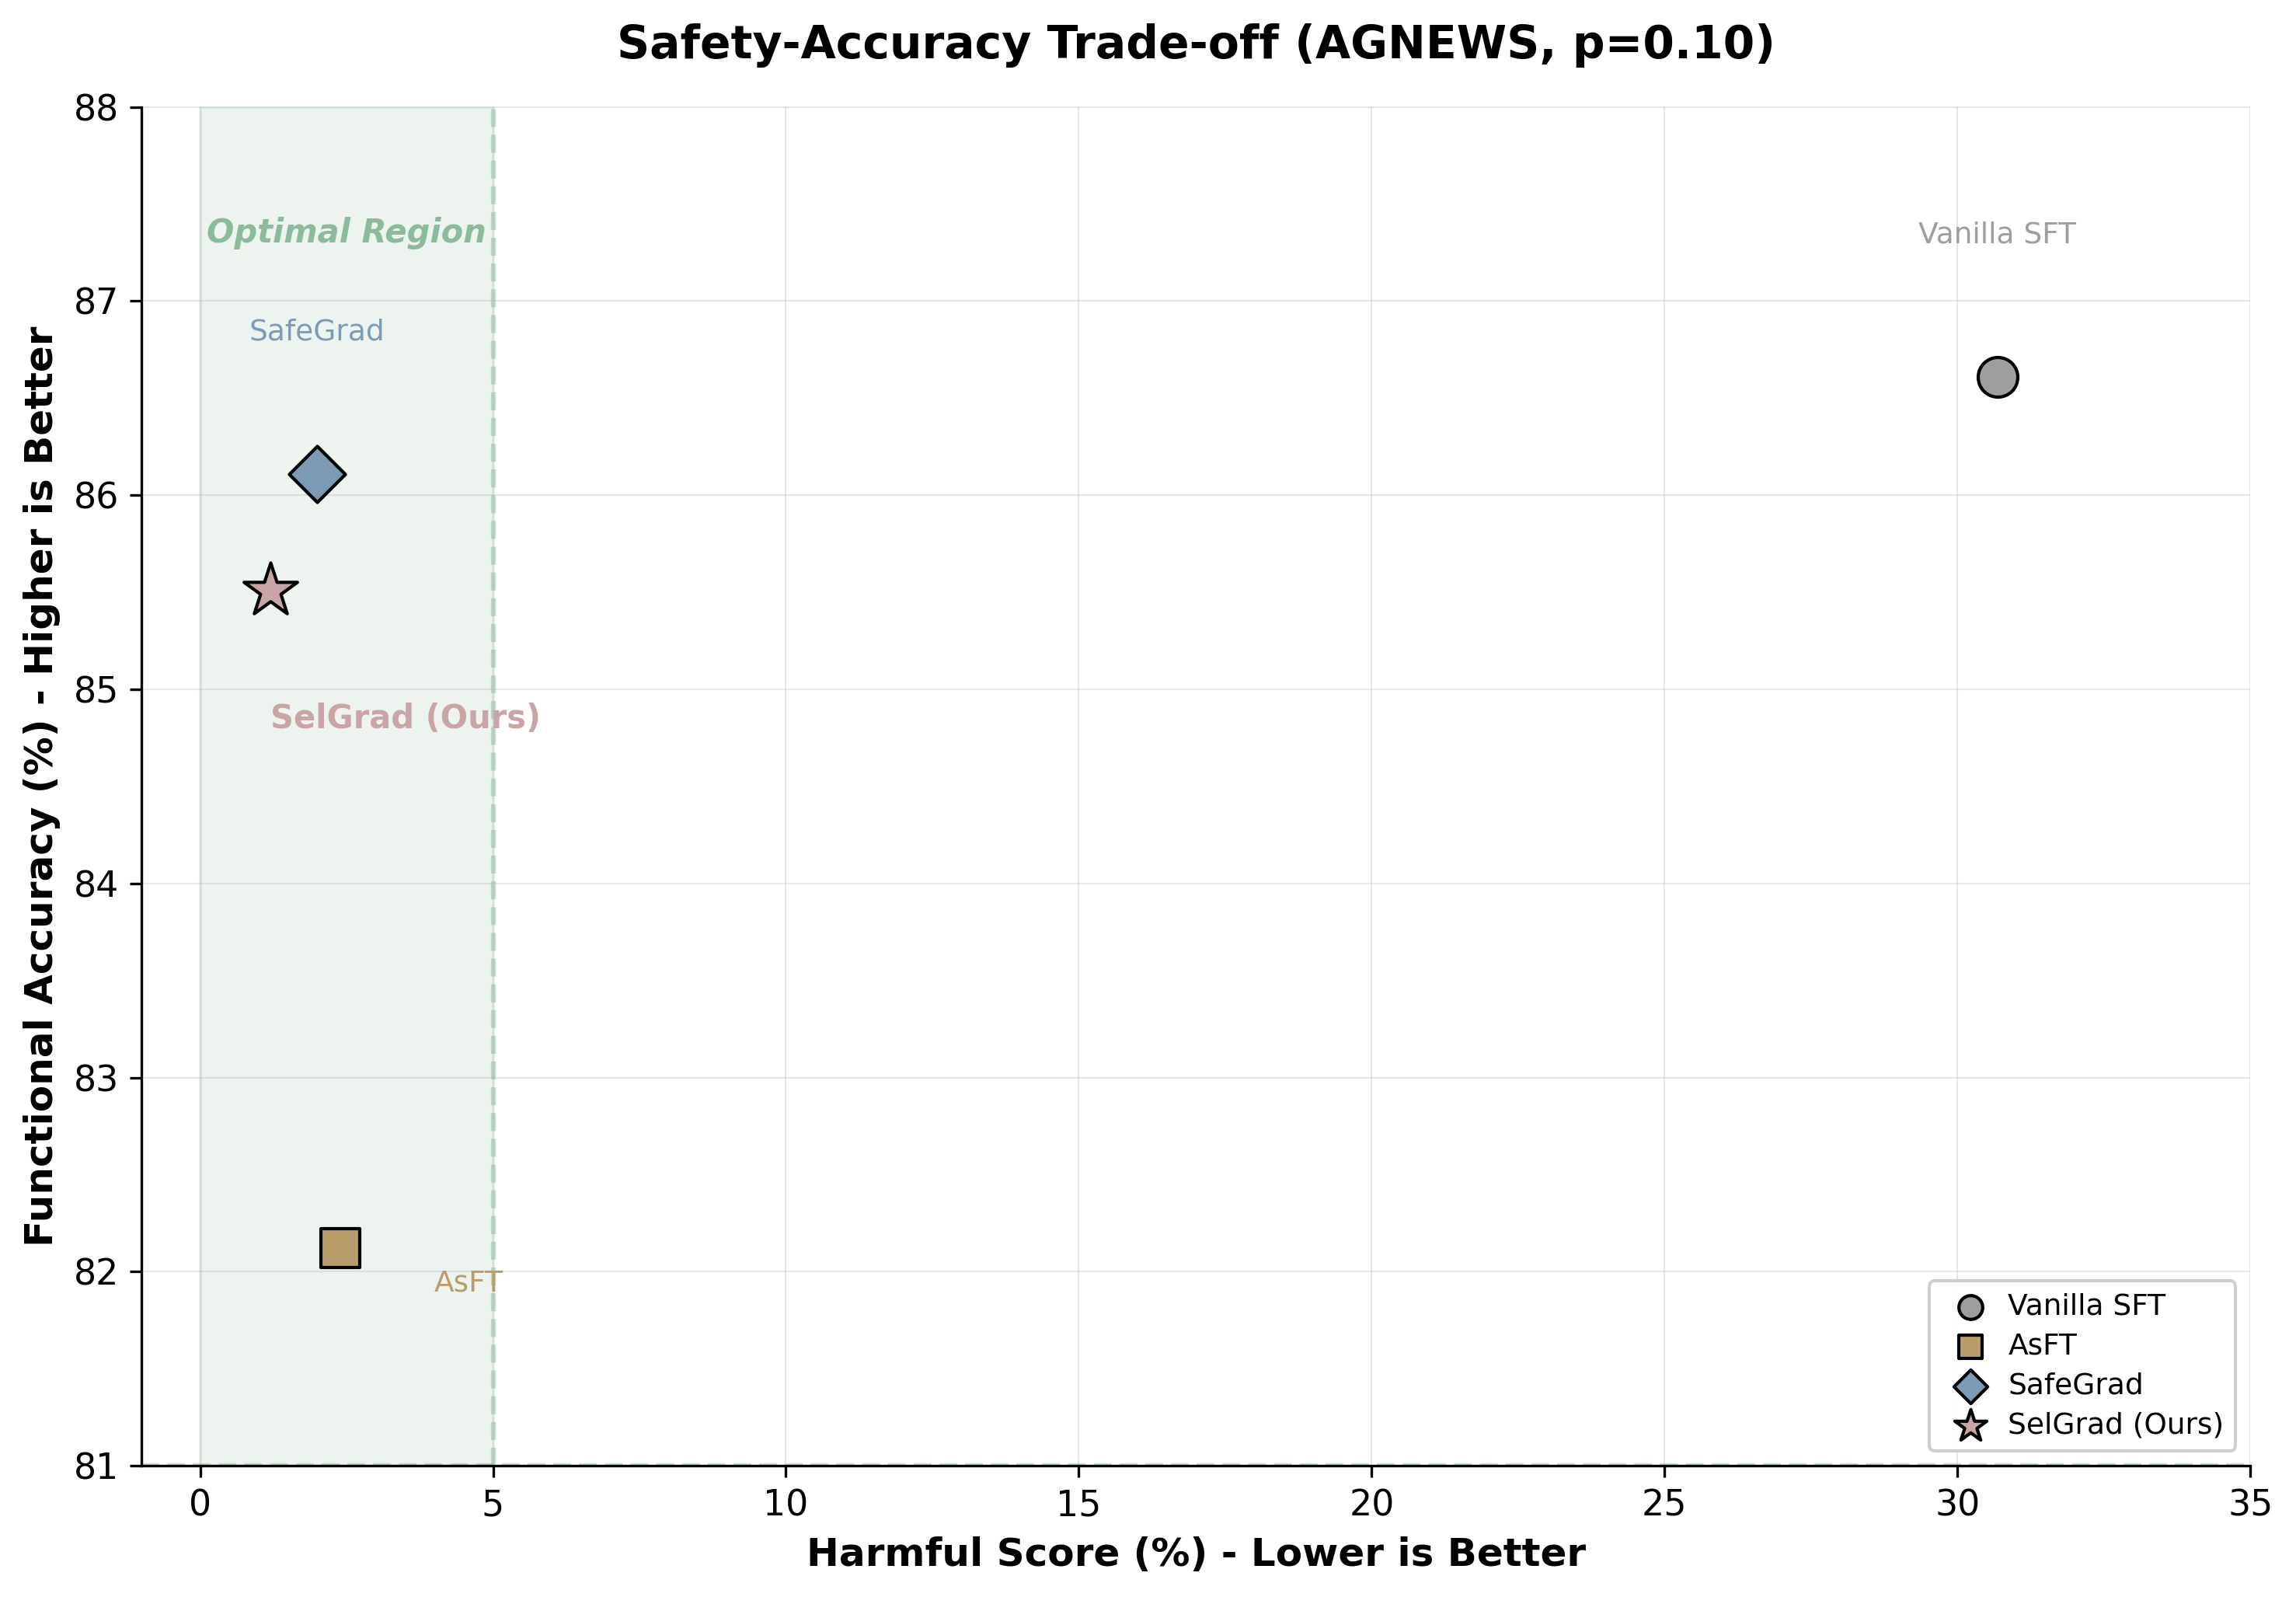
\includegraphics[height=0.73\textheight, keepaspectratio]{figures/fig10_safety_accuracy.png}
\end{center}
\takeaway{SelGrad sits in the optimal region (top-left): lowest HS and highest FA simultaneously.}
\end{frame}

% --- Slide: Efficiency (MERGED: Time + VRAM side by side) ---
\begin{frame}{Efficiency: Training Time \& VRAM}
\vspace{2pt}
\begin{columns}[c]
\column{0.48\textwidth}
\begin{center}
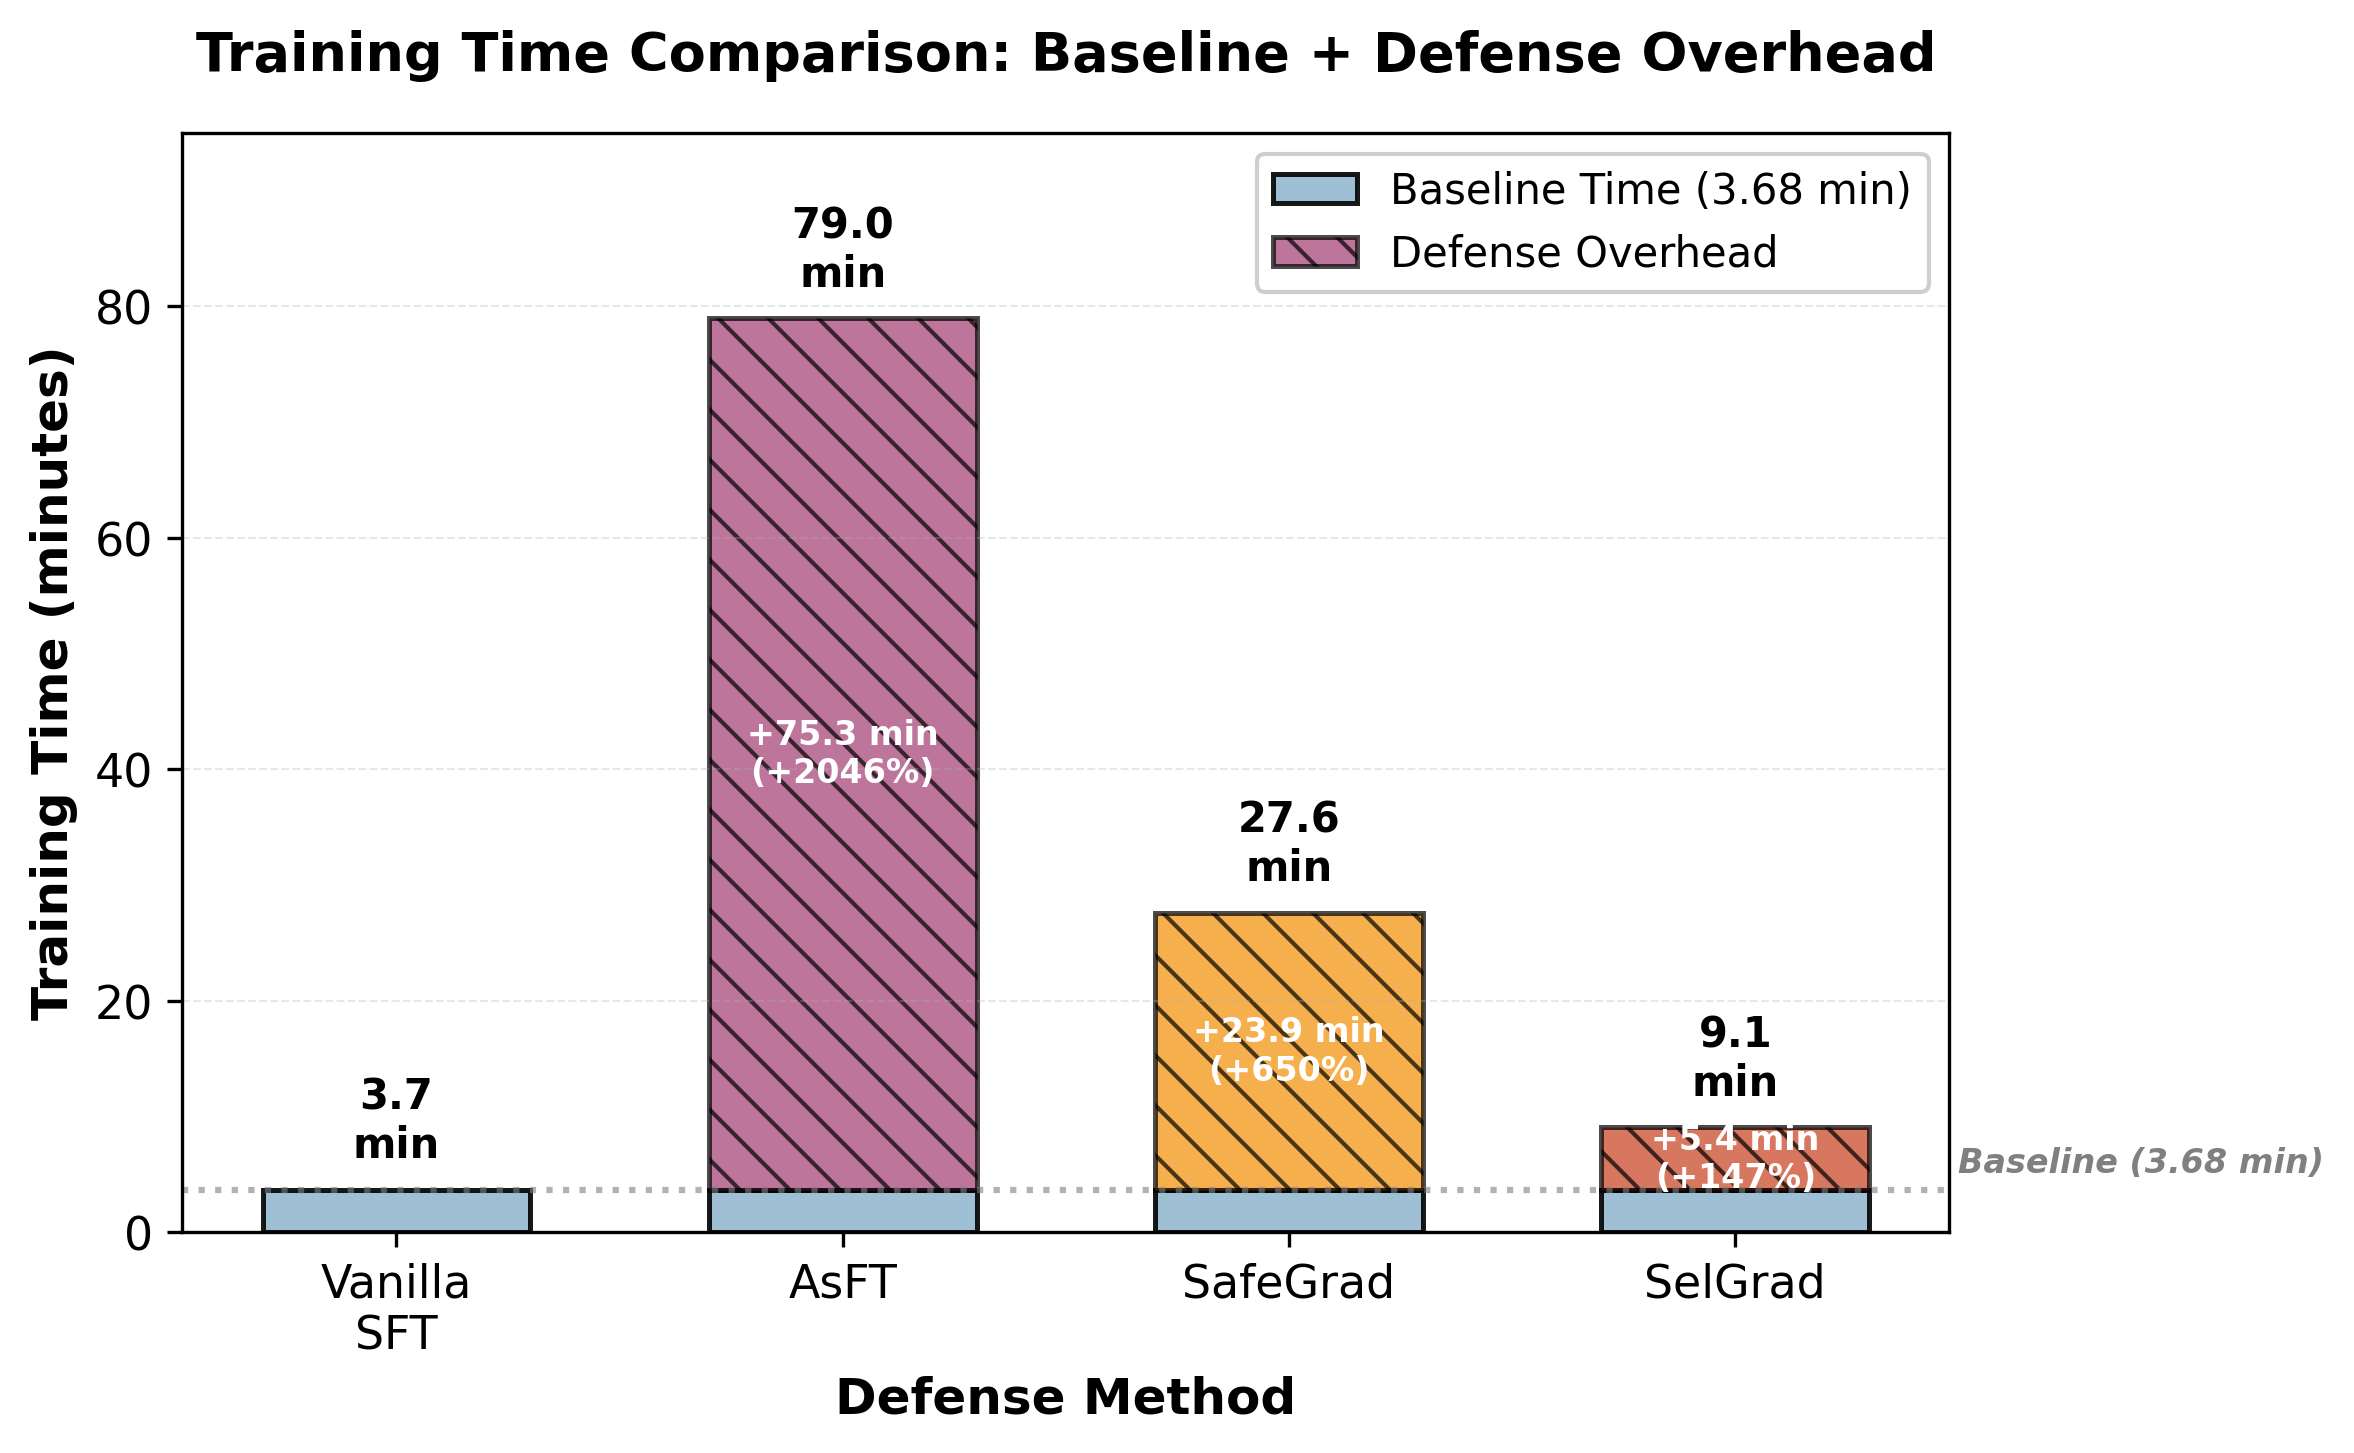
\includegraphics[width=\textwidth, keepaspectratio]{figures/fig12_time_comparison.png}
\end{center}

\column{0.48\textwidth}
\begin{center}
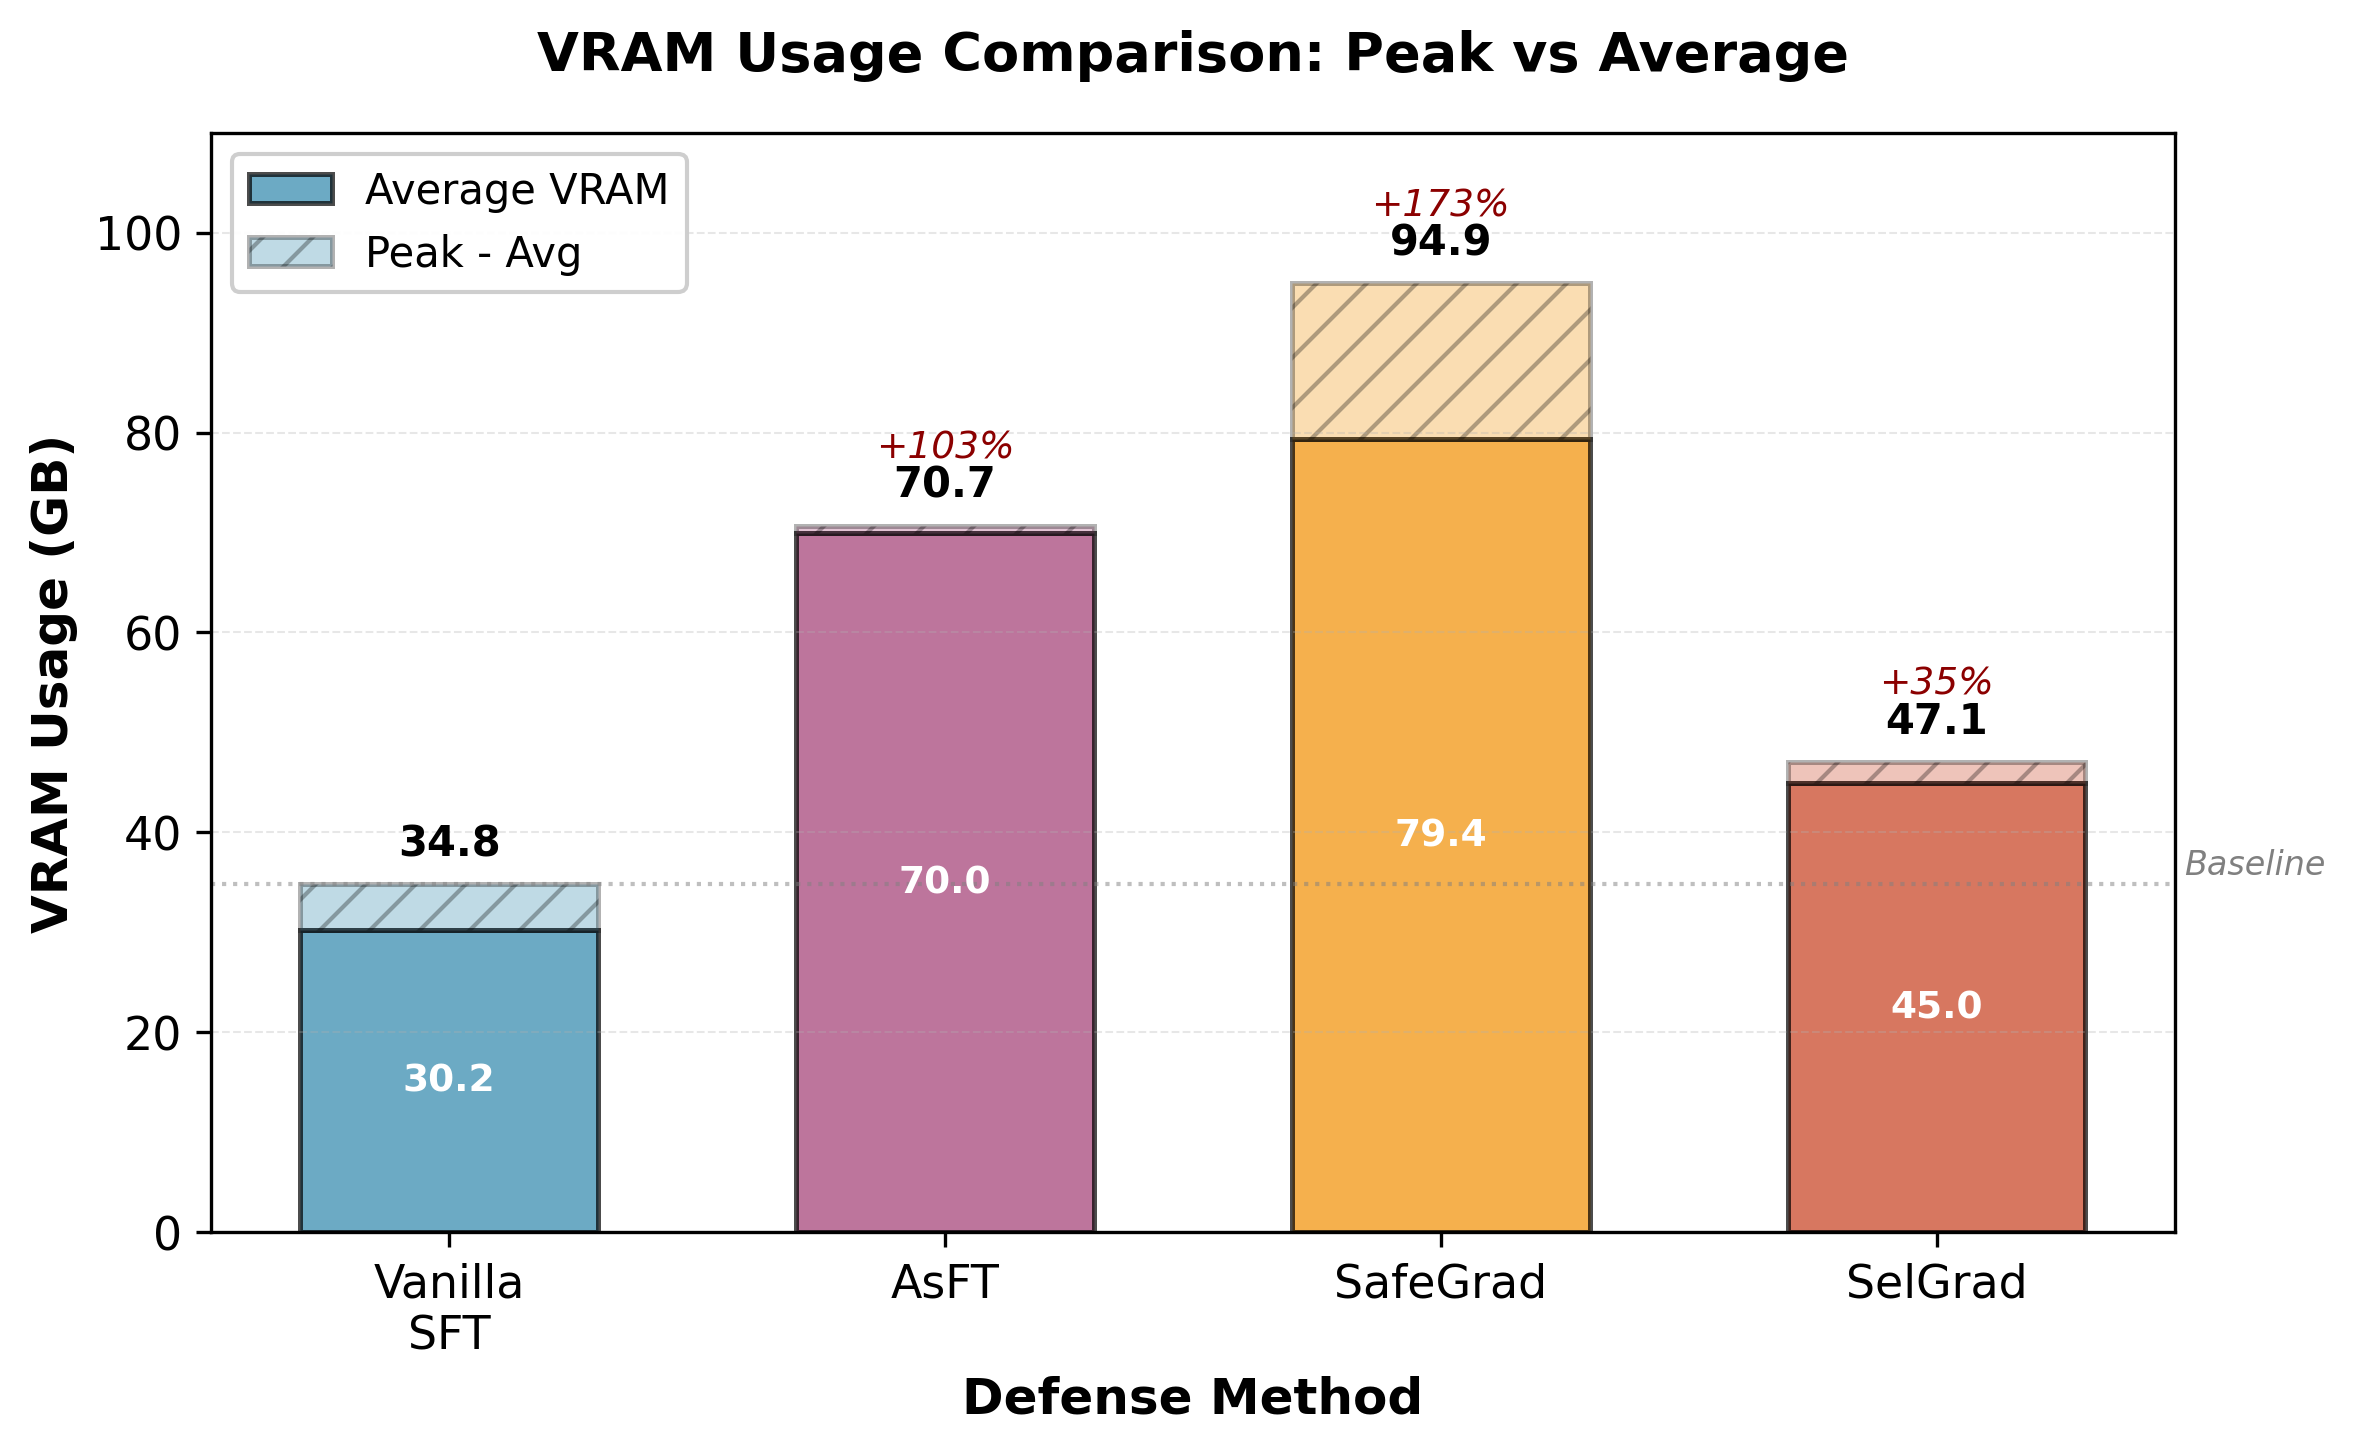
\includegraphics[width=\textwidth, keepaspectratio]{figures/fig13_vram_comparison.png}
\end{center}
\end{columns}
\takeaway{SelGrad adds only 5.4 min overhead (28.3\% of samples undergo surgery vs.\ 100\%). LoRA toggle eliminates the 13.5 GB reference model copy.}
\end{frame}

% --- Slide: Efficiency Summary (KEEP) ---
\begin{frame}{Efficiency Summary}
\vspace{6pt}
\centering
{\small Overhead \% = relative to Vanilla SFT baseline (3.68 min, 34.8 GB)}
\vspace{4pt}
\begin{center}
\renewcommand{\arraystretch}{1.5}
\large
\begin{tabular}{lcccc}
\toprule
\textbf{Method} & \textbf{Time} & \textbf{VRAM} & \textbf{Time OH} & \textbf{VRAM OH} \\
\midrule
Vanilla SFT & 3.68 min & 34.8 GB & --- & --- \\
AsFT & 79.0 min & 70.7 GB & +2046\% & +103\% \\
SafeGrad & 27.6 min & 94.9 GB & +650\% & +173\% \\
\rowcolor{green!10}
\textbf{SelGrad} & \textbf{9.1 min} & \textbf{47.1 GB} & \textbf{+147\%} & \textbf{+35\%} \\
\bottomrule
\end{tabular}
\end{center}
\takeaway{SelGrad is 3$\times$ faster than SafeGrad and uses 50\% less VRAM. The efficiency gain comes primarily from selectivity (28\% vs.\ 100\%), not just the LoRA trick.}
\end{frame}

% --- Slide: Robustness: Attack Types (KEEP) ---
\begin{frame}{Robustness: Different Attack Types}
\vspace{6pt}
\centering
\renewcommand{\arraystretch}{1.3}
\begin{tabular}{lcc|cc|cc|cc}
\toprule
& \multicolumn{2}{c}{\textbf{Harmful}} & \multicolumn{2}{c}{\textbf{AdvBench}} & \multicolumn{2}{c}{\textbf{HarmBench}} & \multicolumn{2}{c}{\textbf{Average}} \\
\textbf{Method} & HS & FA & HS & FA & HS & FA & HS & FA \\
\midrule
SFT & 18.2 & 84.3 & 19.4 & 84.1 & 16.8 & 84.5 & 18.1 & 84.3 \\
AsFT & 4.8 & 84.3 & 5.6 & 83.9 & 3.2 & 84.7 & 4.5 & 84.3 \\
SafeGrad & 4.2 & 83.5 & 4.8 & 83.2 & 2.8 & 83.9 & 3.9 & 83.5 \\
\rowcolor{green!10}
\textbf{SelGrad} & \textbf{2.0} & \textbf{85.9} & \textbf{2.0} & \textbf{85.2} & \textbf{2.4} & \textbf{85.5} & \textbf{2.1} & \textbf{85.5} \\
\bottomrule
\end{tabular}
\takeaway{Loss-based detection generalizes across 3 different backdoor attack types --- not specific to any single attack pattern.}
\end{frame}

% --- Slide: Cross-Dataset (KEEP table, cut figure) ---
\begin{frame}{Cross-Dataset Generalization ($p{=}0.10$)}
\vspace{4pt}
\centering
\small
\renewcommand{\arraystretch}{1.15}
\begin{tabular}{lcc|cc|cc|cc}
\toprule
& \multicolumn{2}{c}{\textbf{SST-2}} & \multicolumn{2}{c}{\textbf{AGNEWS}} & \multicolumn{2}{c}{\textbf{GSM8K}} & \multicolumn{2}{c}{\textbf{Average}} \\
\textbf{Method} & HS$\downarrow$ & FA$\uparrow$ & HS$\downarrow$ & FA$\uparrow$ & HS$\downarrow$ & FA$\uparrow$ & HS$\downarrow$ & FA$\uparrow$ \\
\midrule
SFT & 48.0 & 94.5 & 17.6 & 84.3 & 56.0 & 23.8 & 40.5 & 67.5 \\
Lisa-base & 27.6 & 96.9 & 27.2 & 73.5 & 35.2 & 24.0 & 30.0 & 64.8 \\
Lisa-aligned & 5.6 & 93.6 & 16.8 & 81.8 & 16.0 & 19.4 & 12.8 & 64.9 \\
SafeInstr & 9.2 & 93.4 & 16.8 & 84.3 & 17.6 & 19.3 & 14.5 & 65.7 \\
BEA & 7.2 & 91.6 & 16.4 & 84.4 & 38.8 & 21.0 & 20.8 & 65.7 \\
Safe LoRA & 11.2 & 89.2 & 5.6 & 81.2 & 36.0 & 23.6 & 17.6 & 64.7 \\
AsFT & 3.2 & 94.5 & 4.0 & 84.3 & 14.4 & 26.0 & 7.2 & 68.3 \\
SafeGrad & 2.8 & 93.3 & 3.6 & 83.5 & 13.8 & 24.8 & 6.7 & 67.2 \\
\rowcolor{green!10}
\textbf{SelGrad} & 3.2 & \textbf{93.9} & \textbf{1.6} & \textbf{86.0} & \textbf{12.0} & \textbf{26.2} & \textbf{5.6} & \textbf{68.7} \\
\bottomrule
\end{tabular}
\takeaway{SelGrad outperforms SafeGrad on both metrics across classification (SST-2, AGNEWS) and reasoning (GSM8K) tasks.}
\end{frame}

% --- Slide: Cross-Architecture (MERGED with architecture-dependent analysis) ---
\begin{frame}{Cross-Architecture Evaluation}
\vspace{4pt}
\centering
\renewcommand{\arraystretch}{1.3}
\begin{tabular}{lcccccccc}
\toprule
& \multicolumn{2}{c}{\textbf{Llama-2-7B}} & \multicolumn{2}{c}{\textbf{Llama-3-8B}} & \multicolumn{2}{c}{\textbf{Qwen-2-7B}} & \multicolumn{2}{c}{\textbf{Gemma-2-9B}} \\
\textbf{Method} & FA & HS & FA & HS & FA & HS & FA & HS \\
\midrule
SFT & 84.3 & 17.6 & 90.3 & 73.6 & 90.3 & 49.2 & 88.3 & 32.0 \\
AsFT & 84.3 & 4.0 & 92.3 & 15.2 & 87.9 & 5.2 & 86.6 & 6.0 \\
SafeGrad & 84.8 & 3.2 & 84.8 & 3.2 & 85.6 & 2.9 & 87.0 & 4.0 \\
\rowcolor{green!10}
\textbf{SelGrad} & \textbf{85.3} & \textbf{2.0} & 89.5 & 6.4 & 82.4 & \textbf{2.8} & \textbf{89.7} & \textbf{2.0} \\
\bottomrule
\end{tabular}

\vspace{8pt}
\begin{columns}[T]
\column{0.48\textwidth}
\begin{exampleblock}{\small Strong: Llama-2, Gemma-2 ($D_{KL} > 1.5$)}
\small Well-separated loss distributions. Best-in-class on both: HS $\leq 2.0\%$.
\end{exampleblock}

\column{0.48\textwidth}
\begin{alertblock}{\small Challenging: Llama-3 ($D_{KL} \approx 0.8$)}
\small HS=6.4\% (vs SafeGrad 3.2\%). Llama-3's pre-training generalizes trigger patterns better $\Rightarrow$ reduced loss separability. Still below 10\% safety threshold; FA is 89.5\% vs.\ SafeGrad's 84.8\%.
\end{alertblock}
\end{columns}
\end{frame}

% ══════════════════════════════════════════════════════════════
\section{Conclusion \& Future Work}
% ══════════════════════════════════════════════════════════════
\sectionslide{Conclusion \& Future Work}{Summary of contributions and research directions}

% --- Slide: Summary of Contributions (ENHANCED) ---
\begin{frame}{Summary of Contributions}
\vspace{4pt}
\centering
{\small\textbf{Gap:} No prior method achieves low HS, high FA, and low cost simultaneously.}

\vspace{10pt}
\begin{columns}[c]
\column{0.30\textwidth}
\centering
{\Huge\textcolor{safegreen}{\textbf{3$\times$}}}\\[4pt]
{\large faster training}\\[2pt]
9.1 vs 27.6 min\\[6pt]
{\footnotesize\textcolor{gray}{Selective Defense:\\surgery on 28\%, not 100\%}}

\column{0.30\textwidth}
\centering
{\Huge\textcolor{safegreen}{\textbf{50\%}}}\\[4pt]
{\large less VRAM}\\[2pt]
47.1 vs 94.9 GB\\[6pt]
{\footnotesize\textcolor{gray}{LoRA-based KL:\\42 MB vs 13.5 GB copy}}

\column{0.30\textwidth}
\centering
{\Huge\textcolor{safegreen}{\textbf{2.39\%}}}\\[4pt]
{\large harmful score}\\[2pt]
vs SafeGrad 3.60\%\\[6pt]
{\footnotesize\textcolor{gray}{Loss-based Detection:\\lowest across 9 methods}}
\end{columns}

\vspace{12pt}
\centering
Validated: 3 datasets $\times$ 4 architectures $\times$ poison ratios 0.05--0.20 $\times$ 3 attack types
\end{frame}

% --- Slide: Deployment Guidelines (MOVED from Discussion) ---
\begin{frame}{Deployment Guidelines}
\vspace{8pt}
\begin{columns}[T]
\column{0.48\textwidth}
\begin{alertblock}{Boundary Conditions}
\begin{itemize}
  \item Adversarial triggers mimicking benign loss\\
        $\Rightarrow$ fall back to uniform defense when $D_{KL} < 0.5$
  \item Long-context tasks have wider loss variance\\
        $\Rightarrow$ token-level detection
\end{itemize}
\end{alertblock}

\column{0.48\textwidth}
\begin{exampleblock}{Architecture Guidelines}
\begin{itemize}
  \item \textbf{Llama-2, Gemma}: default params
  \item \textbf{Llama-3}: multi-signal detection
  \item \textbf{Qwen}: threshold calibration
  \item \textbf{New arch}: check $D_{KL}$ on 100 samples
\end{itemize}
\end{exampleblock}
\end{columns}
\takeaway{SelGrad includes a built-in diagnostic: if $D_{KL}$ between benign and suspicious loss distributions is below 0.5, automatically fall back to uniform defense for safety.}
\end{frame}

% --- Slide: Future Work (TIGHTENED) ---
\begin{frame}{Future Work}
\vspace{10pt}
\begin{enumerate}
  \item \textbf{Multi-Signal Detection}\\
  {\small Integrate activation clustering, gradient norms, and attention anomalies --- directly addresses the Llama-3 limitation where loss separation alone is insufficient.}

  \vspace{8pt}
  \item \textbf{Adaptive Defense Parameters}\\
  {\small Meta-learning optimal $(w_p, \rho_p)$ from task characteristics; online optimization of thresholds without fixed target ranges.}

  \vspace{8pt}
  \item \textbf{Adversarial-Aware Detection}\\
  {\small Defense against loss-mimicking attacks where adversaries deliberately craft triggers that produce benign-like losses --- the fundamental limitation of loss-based detection.}

  \vspace{8pt}
  \item \textbf{Cross-Architecture Scaling}\\
  {\small Models $>$30B parameters, full fine-tuning (not just LoRA), Mixture-of-Experts, and quantized models (4/8-bit).}
\end{enumerate}
\end{frame}

% ══════════════════════════════════════════════════════════════
% THANK YOU
% ══════════════════════════════════════════════════════════════
{
\setbeamertemplate{footline}{}
\begin{frame}[plain]
\begin{tikzpicture}[remember picture, overlay]
  \fill[dividerblue] (current page.south west) rectangle (current page.north east);
  \fill[accentgold] ([yshift=2pt]current page.south west) rectangle ([yshift=6pt]current page.south east);
  \fill[accentgold] ([yshift=-2pt]current page.north west) rectangle ([yshift=-6pt]current page.north east);
  \node[anchor=center, text=white] at ([yshift=20pt]current page.center) {{\fontsize{36}{42}\selectfont\bfseries Thank You}};
  \node[anchor=center, text=white!80] at ([yshift=-15pt]current page.center) {{\Large Questions \& Discussion}};
  \node[anchor=center, text=white!60] at ([yshift=-45pt]current page.center) {{\normalsize Wei-Cheng Chiu \quad $\mid$ \quad m11315038@mail.ntust.edu.tw}};
\end{tikzpicture}
\end{frame}
}

% ══════════════════════════════════════════════════════════════
% BACKUP SLIDES
% ══════════════════════════════════════════════════════════════
\appendix
\newcounter{backupslide}
\setcounter{backupslide}{\value{framenumber}}

{
\setbeamertemplate{footline}{}
\begin{frame}[plain]
\begin{tikzpicture}[remember picture, overlay]
  \fill[dividerblue] (current page.south west) rectangle (current page.north east);
  \fill[accentgold] ([yshift=2pt]current page.south west) rectangle ([yshift=6pt]current page.south east);
  \fill[accentgold] ([yshift=-2pt]current page.north west) rectangle ([yshift=-6pt]current page.north east);
  \node[anchor=center, text=white] at ([yshift=10pt]current page.center) {{\fontsize{28}{34}\selectfont\bfseries Backup Slides}};
  \node[anchor=center, text=white!70] at ([yshift=-20pt]current page.center) {{\large For committee Q\&A}};
\end{tikzpicture}
\end{frame}
}

% --- Backup 1: Loss Distribution Histograms ---
\begin{frame}{Backup: Loss Distributions per Architecture}
\begin{center}
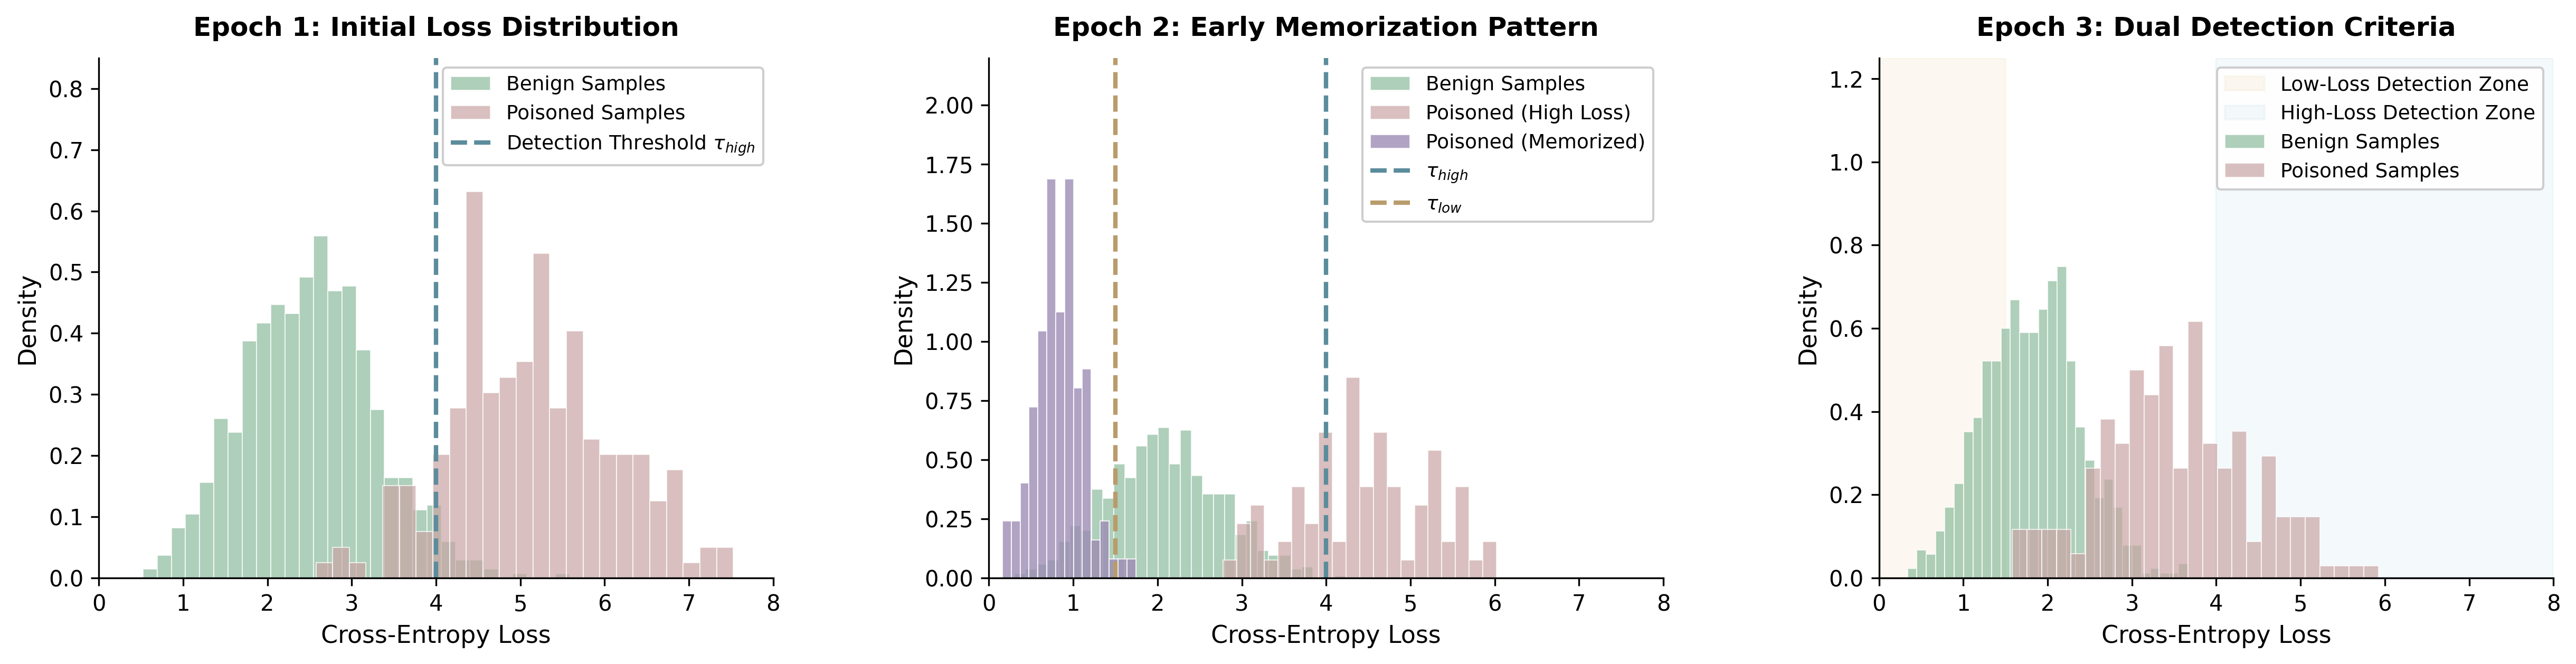
\includegraphics[width=0.95\textwidth, keepaspectratio]{figures/fig05_loss_distribution.png}
\end{center}
\takeaway{Benign ($\mu{=}2.1$) vs.\ poisoned ($\mu{=}5.3$) loss distributions show clear separation on Llama-2. On Llama-3, $D_{KL}$ drops to $\approx 0.8$, explaining the reduced detection accuracy.}
\end{frame}

% --- Backup 2: Gradient Projection Visualization ---
\begin{frame}{Backup: Gradient Projection Visualization}
\begin{center}
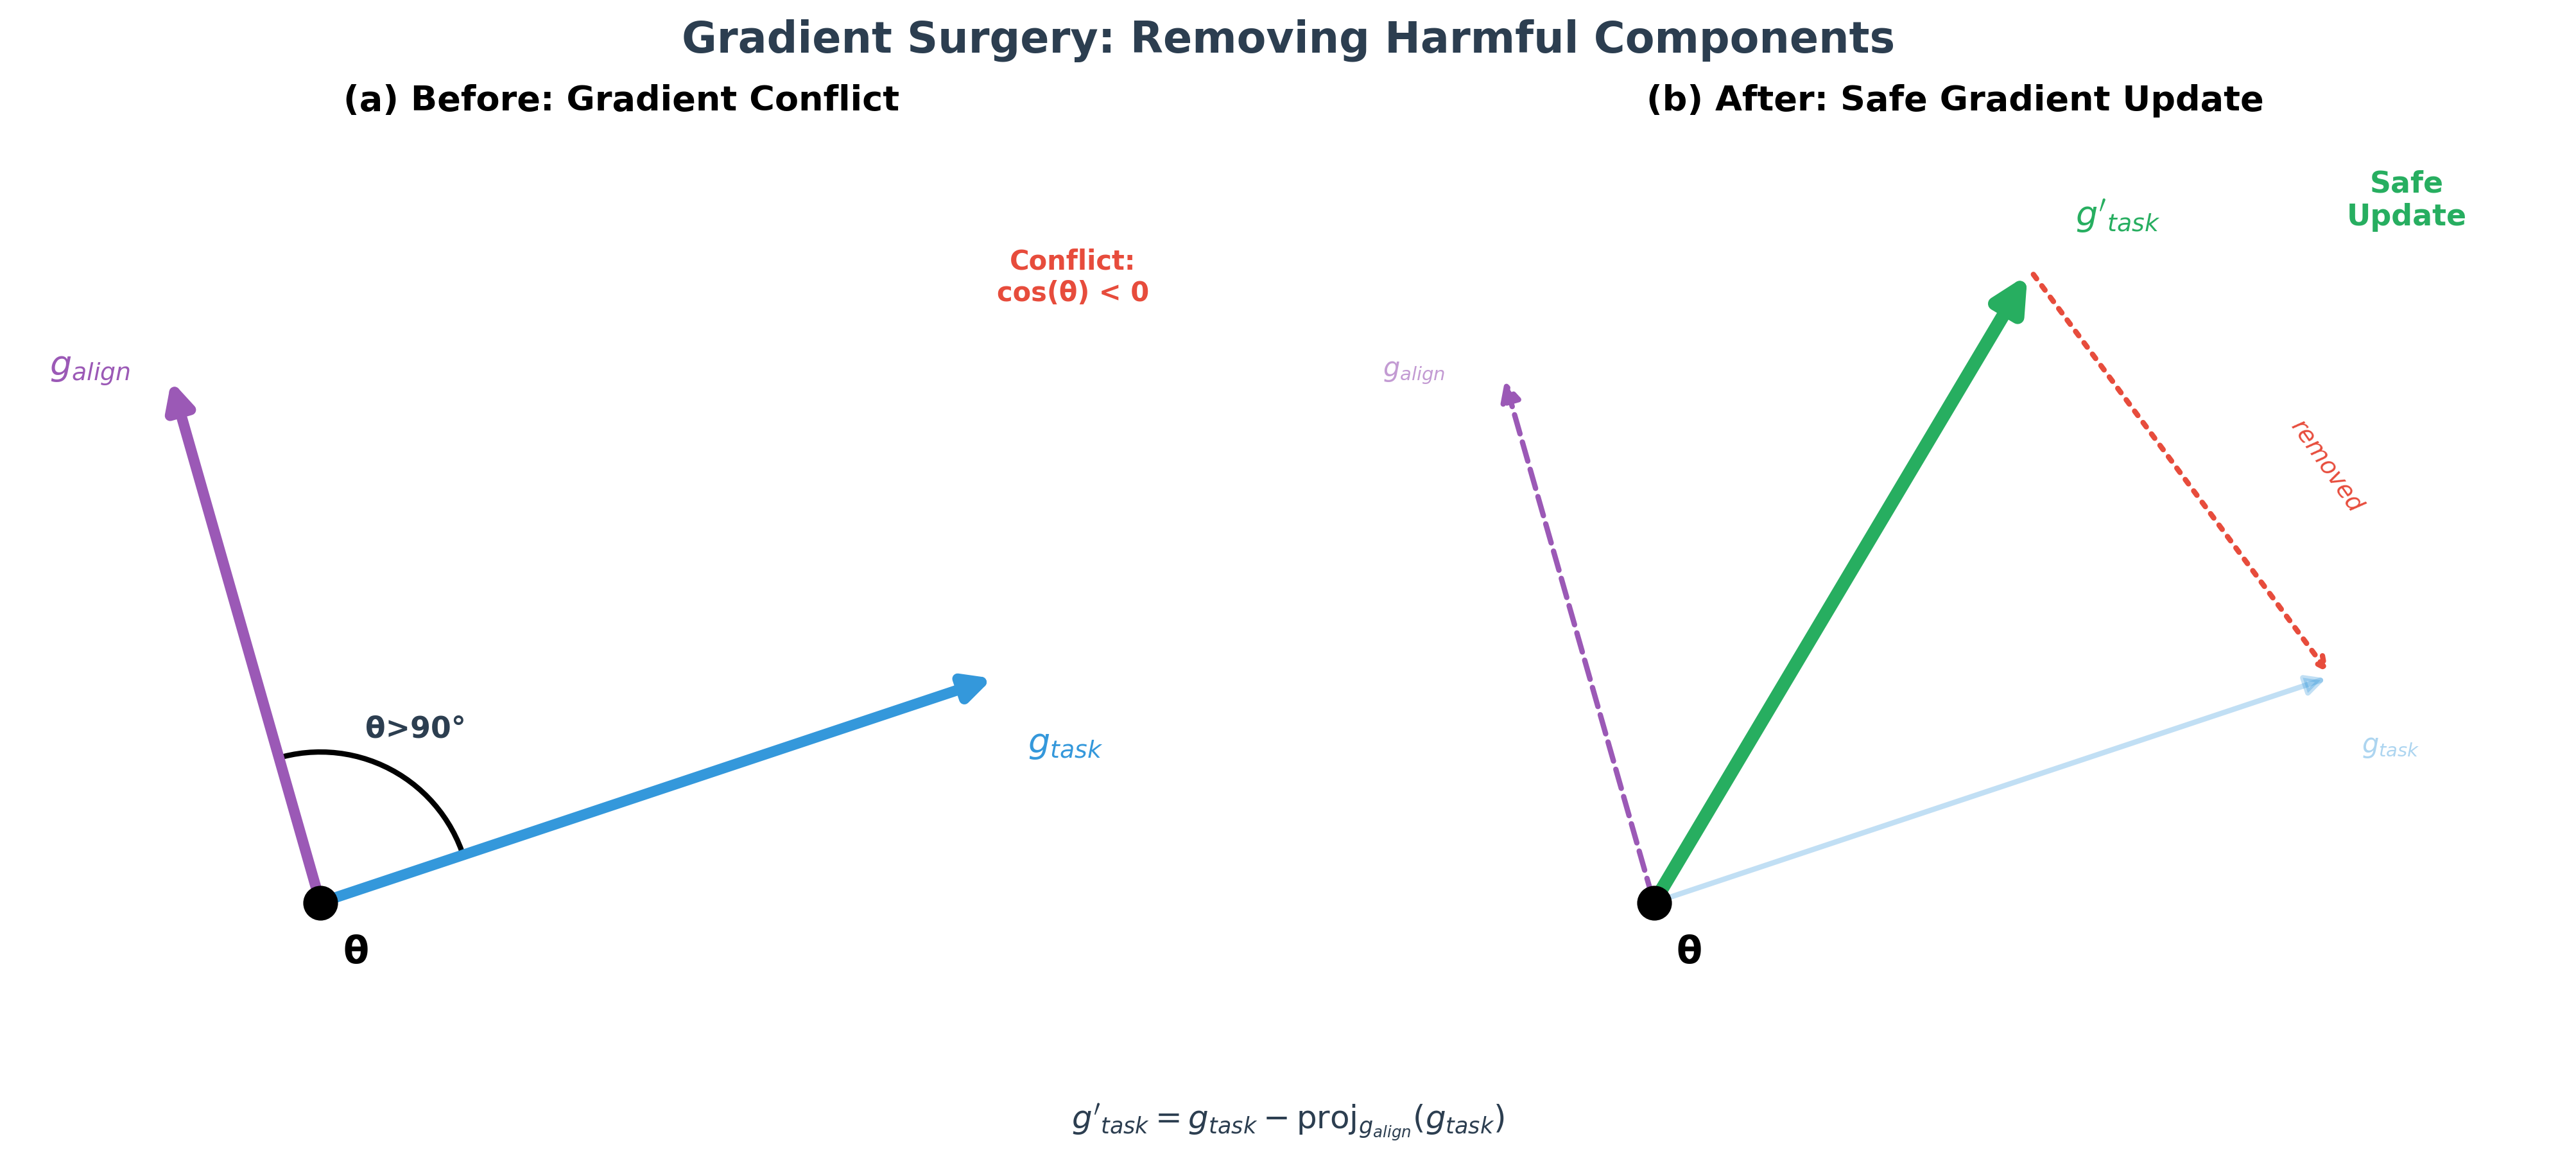
\includegraphics[width=0.85\textwidth, keepaspectratio]{figures/fig07_gradient_projection.png}
\end{center}
\takeaway{The projection $g'_{\text{task}} = g_{\text{task}} - \text{proj}_{g_{\text{align}}}(g_{\text{task}})$ removes the anti-safety component while preserving the task-useful direction.}
\end{frame}

% --- Backup 3: HS Heatmap (moved from main) ---
\begin{frame}{Backup: Harmful Score Heatmap \& Efficiency}
\begin{center}
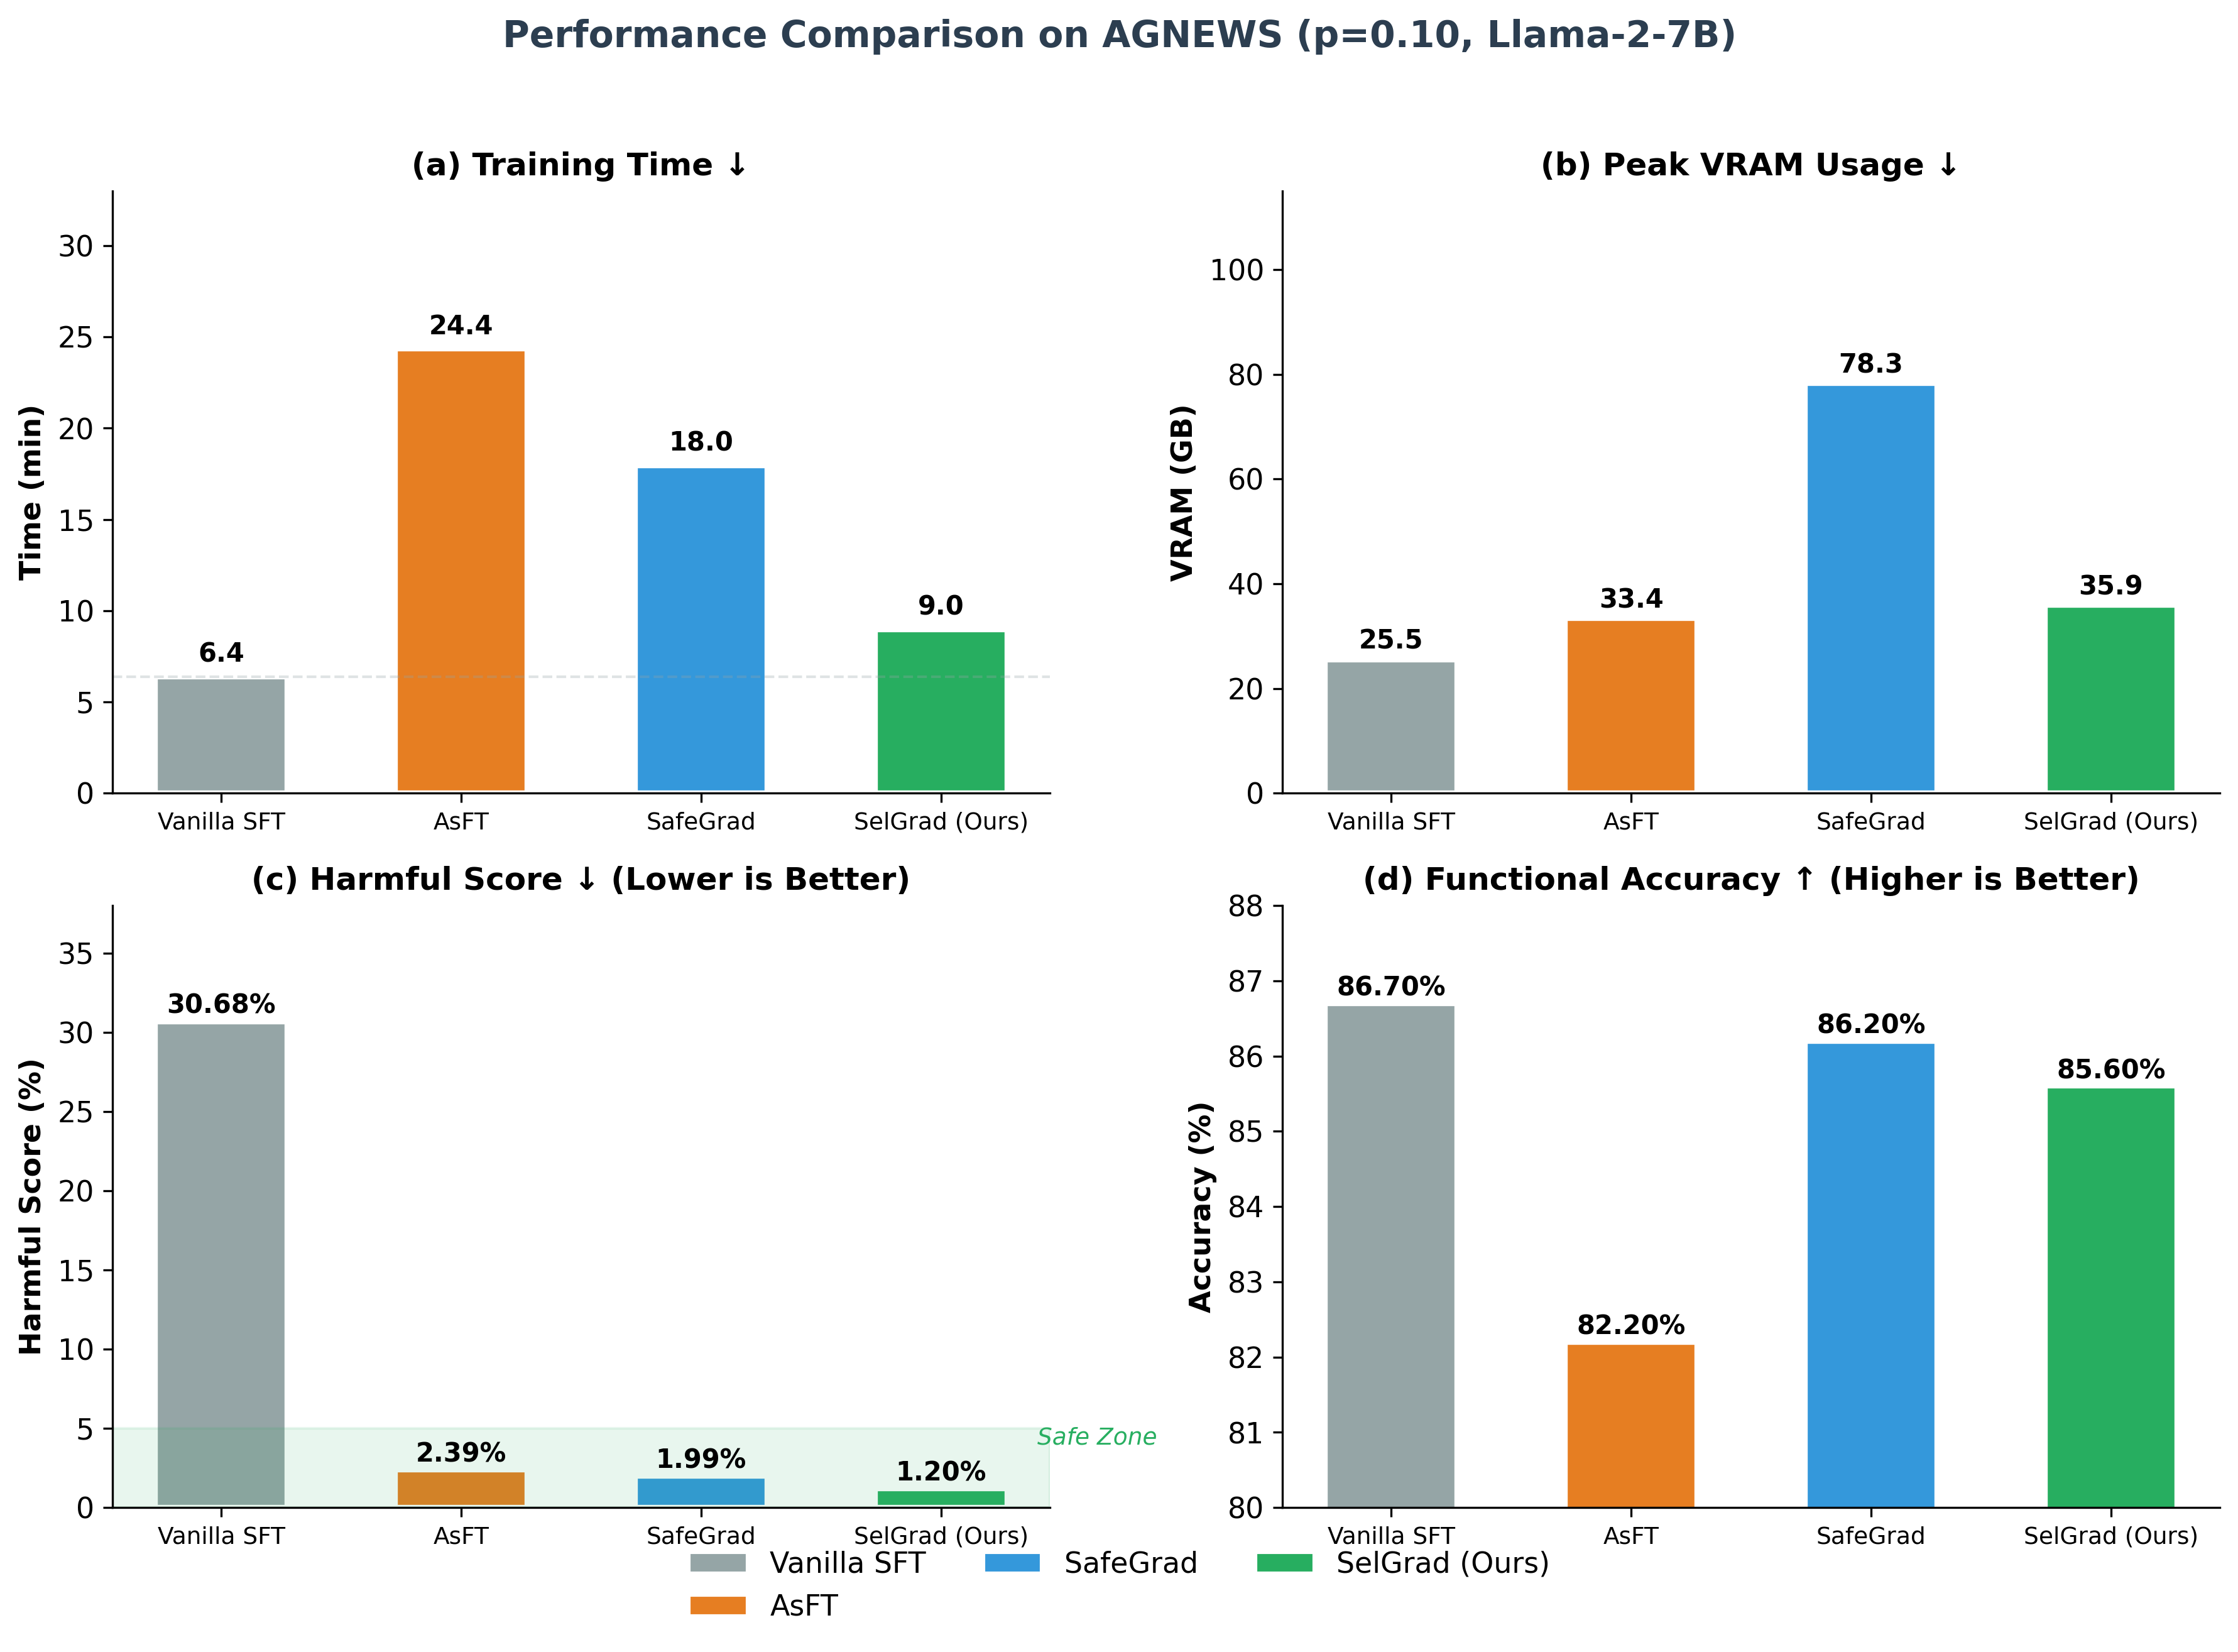
\includegraphics[height=0.80\textheight, keepaspectratio]{figures/fig09_fair_baseline.png}
\end{center}
\end{frame}

% --- Backup 4: Performance Comparison (moved from main) ---
\begin{frame}{Backup: Detailed Performance Comparison (AGNEWS, $p{=}0.10$)}
\begin{center}
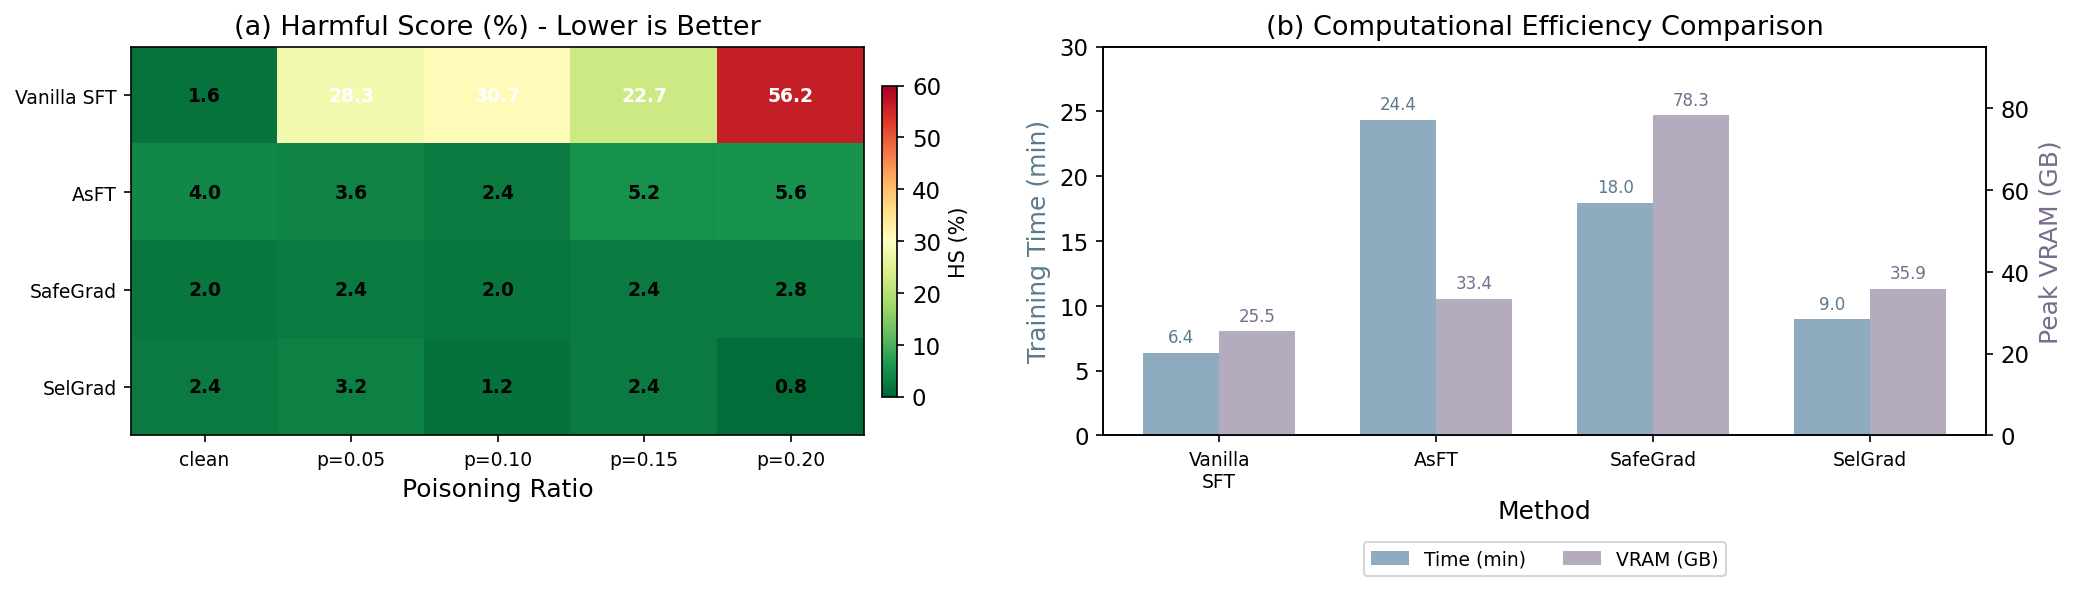
\includegraphics[width=0.95\textwidth, keepaspectratio]{figures/fig11_method_comparison.png}
\end{center}
\end{frame}

% --- Backup 5: Efficiency Scatter (moved from main) ---
\begin{frame}{Backup: Efficiency Trade-off Scatter}
\begin{center}
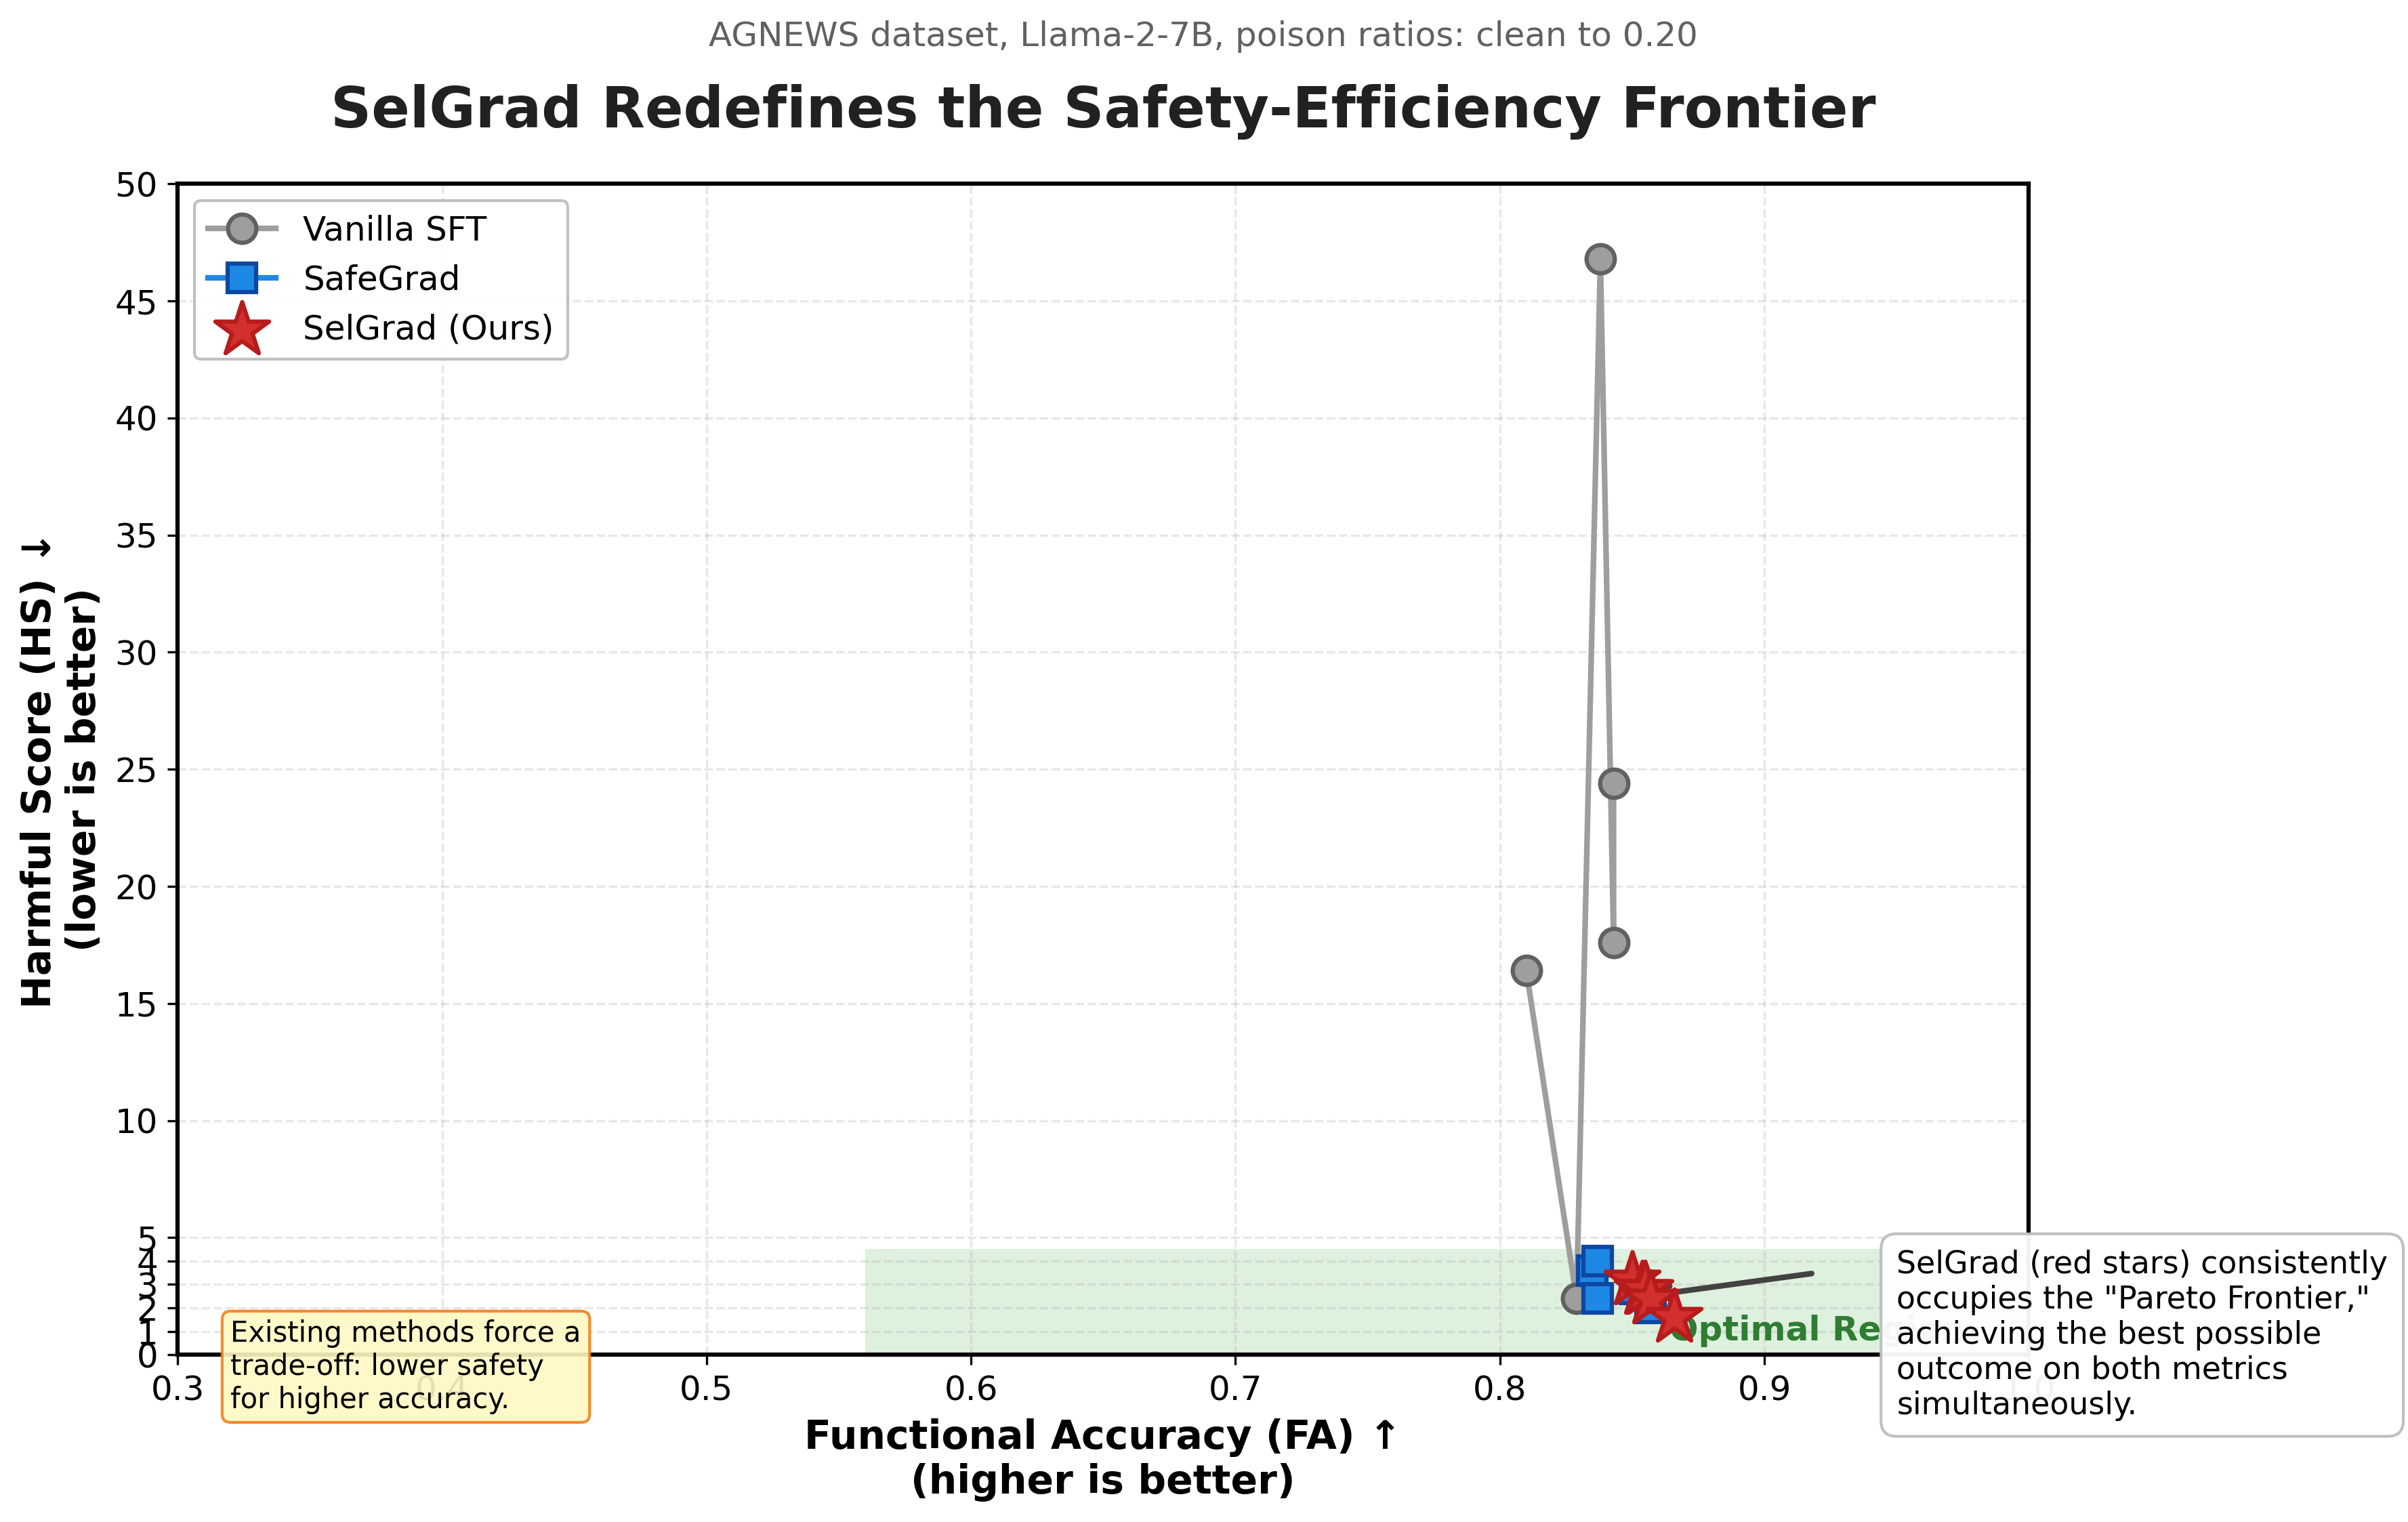
\includegraphics[height=0.70\textheight, keepaspectratio]{figures/fig14_efficiency_tradeoff.png}
\end{center}
\takeaway{SelGrad is closest to vanilla SFT while providing strong safety guarantees.}
\end{frame}

% --- Backup 6: Sample Size Robustness (moved from main) ---
\begin{frame}{Backup: Robustness Across Sample Sizes}
\vspace{4pt}
\centering
\small
\renewcommand{\arraystretch}{1.2}
\begin{tabular}{lccccc|c}
\toprule
& \multicolumn{6}{c}{\textbf{Harmful Score $\downarrow$ (\%)}} \\
\textbf{Method} & $n{=}500$ & $n{=}1000$ & $n{=}1500$ & $n{=}2000$ & $n{=}2500$ & \textbf{Avg} \\
\midrule
SFT & 12.40 & 17.60 & 19.20 & 21.80 & 23.60 & 18.92 \\
AsFT & 4.00 & 4.00 & 4.20 & 4.60 & 5.00 & 4.36 \\
SafeGrad & 3.20 & 3.60 & 2.80 & 2.40 & 4.80 & 3.36 \\
\rowcolor{green!10}
\textbf{SelGrad} & \textbf{1.59} & \textbf{2.39} & \textbf{2.50} & 2.80 & \textbf{4.00} & \textbf{2.66} \\
\bottomrule
\end{tabular}

\vspace{6pt}

\begin{tabular}{lccccc|c}
\toprule
& \multicolumn{6}{c}{\textbf{Finetune Accuracy $\uparrow$ (\%)}} \\
\textbf{Method} & $n{=}500$ & $n{=}1000$ & $n{=}1500$ & $n{=}2000$ & $n{=}2500$ & \textbf{Avg} \\
\midrule
AsFT & 84.10 & 84.30 & 84.20 & 84.40 & 84.30 & 84.26 \\
SafeGrad & 83.30 & 83.60 & 84.00 & 85.00 & 86.00 & 84.38 \\
\rowcolor{green!10}
\textbf{SelGrad} & \textbf{85.21} & 84.62 & \textbf{85.21} & \textbf{87.31} & 85.11 & \textbf{85.49} \\
\bottomrule
\end{tabular}
\end{frame}

% --- Backup 7: Cross-Dataset Generalization Figure ---
\begin{frame}{Backup: Cross-Dataset Generalization (Visual)}
\begin{center}
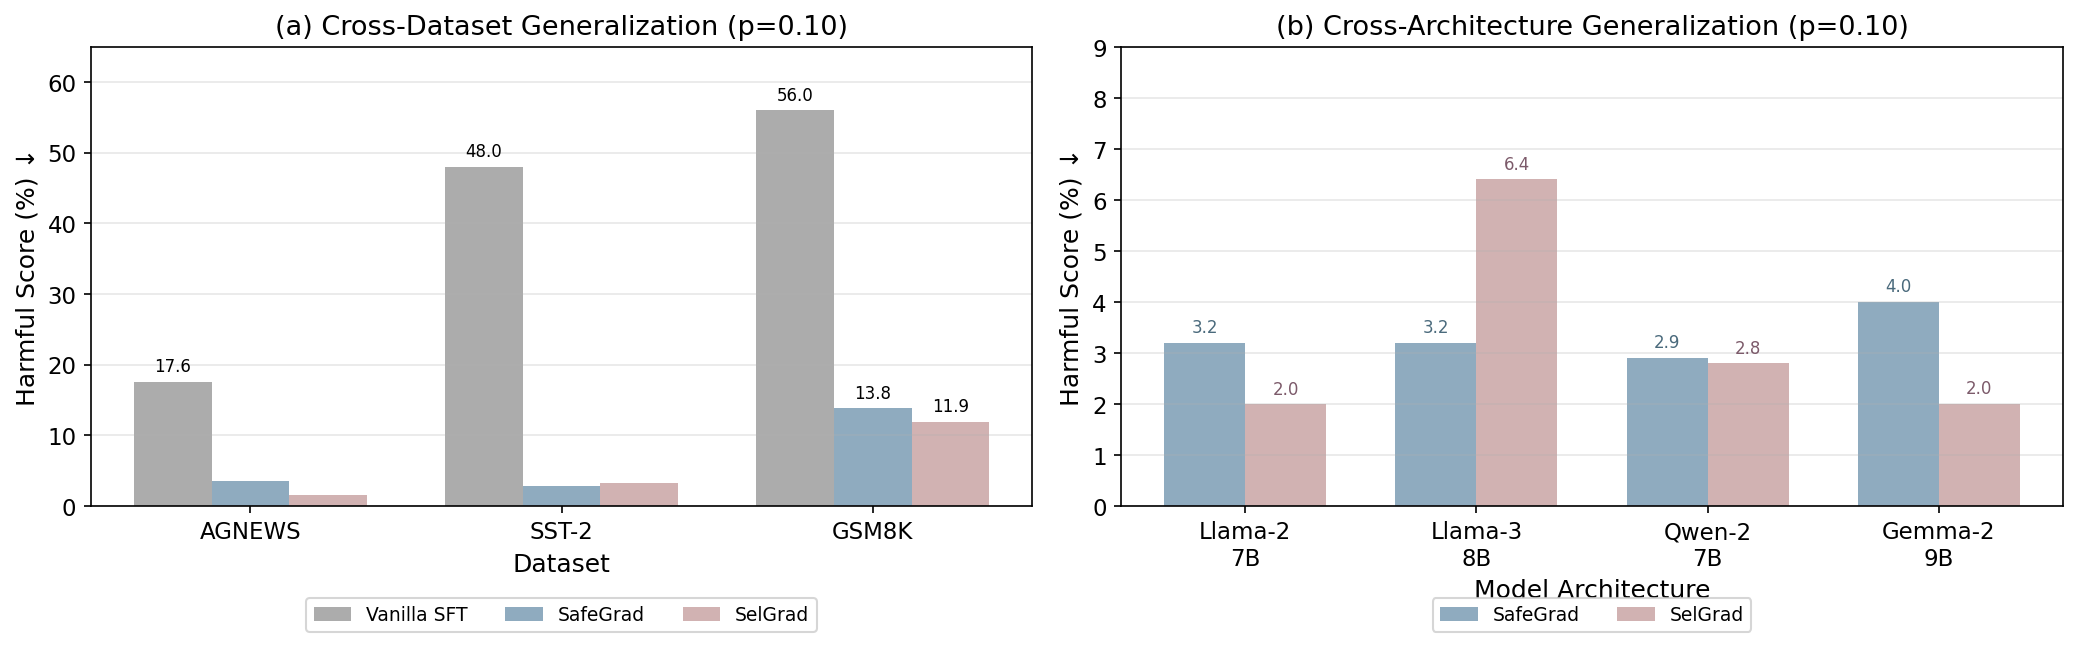
\includegraphics[width=0.92\textwidth, keepaspectratio]{figures/fig15_generalization.png}
\end{center}
\end{frame}

% --- Backup 8: Comparison Fairness Discussion ---
\begin{frame}{Backup: Is the SafeGrad Comparison Fair?}
\vspace{8pt}
\begin{block}{Q: SafeGrad uses a full reference model --- could it also use LoRA?}
\small
Yes, SafeGrad could adopt LoRA-based KL to reduce VRAM. However:
\begin{itemize}
  \item The \textbf{core overhead} --- computing alignment gradients and projections for \textbf{100\% of samples} --- would remain
  \item SelGrad's efficiency gain comes primarily from \textbf{selectivity} (28\% vs 100\%), not just the LoRA trick
  \item Even with LoRA, SafeGrad would still be $\sim$2.5$\times$ slower due to uniform gradient surgery
\end{itemize}
\end{block}

\vspace{8pt}
\begin{exampleblock}{Decomposition of SelGrad's Efficiency Gains}
\small
\begin{itemize}
  \item \textbf{Selectivity} (28\% vs 100\% surgery): accounts for $\sim$70\% of time reduction
  \item \textbf{LoRA-based KL} (42 MB vs 13.5 GB): accounts for $\sim$100\% of VRAM reduction
  \item Both innovations are independent and complementary
\end{itemize}
\end{exampleblock}
\end{frame}

\setcounter{framenumber}{\value{backupslide}}

\end{document}
